\RequirePackage{fix-cm}
\documentclass[conf]{new-aiaa}

\usepackage[utf8]{inputenc}
\usepackage{graphicx}
\usepackage{siunitx}
\sisetup{group-separator = {,}}
\usepackage{booktabs}
\usepackage{enumitem}
\usepackage{float}
\usepackage{amsmath}
\usepackage[version=4]{mhchem}
\usepackage{longtable,tabularx}
\usepackage{placeins}
\usepackage{multirow}
\usepackage{booktabs}
\usepackage{latexsym}
\usepackage{multicol}
\usepackage{subcaption}
\usepackage{hyperref}
\usepackage[sort&compress,numbers]{natbib} % For bibtex \citet, \citep
\usepackage{hypernat} % To get natbib to play nicely with hyperref
\usepackage{doi} % For getting hyperlinked DOI in the references

%% Custom modifications of hyperlinks.
% This is not from the AIAA template standard
\usepackage{xcolor}
\colorlet{mblue}{blue!40!black}
\hypersetup{bookmarksnumbered=true,colorlinks=true,linkcolor=mblue,citecolor=mblue,urlcolor=mblue}

\setlength\LTleft{0pt} 

\hypersetup{
    pdfauthor={Peter Atma}, % insert author here
	pdftitle={Aviation 2023 Paper}, % insert title here
	pdfsubject={Comparing Hydrogen and Jet-A for an N+3 Turbofan with Water Recirculation using Gradient-Based Optimization}, % insert keywords here
}

\graphicspath{{../figures/}}

% [x] TODO: AL-PA, Consider changing the title to "Comparing Hydrogen and Jet-A for an N+3 Turbofan with Water Recirculation using Gradient-Based Optimization"
\title{Comparing Hydrogen and Jet-A for an N+3 Turbofan with Water Recirculation using Gradient-Based Optimization} % change
\author{Peter N.~Atma\footnote{MSE Student, Department of Aerospace Engineering, AIAA Student Member}}
\author{Andrew H~.R.~Lamkin\footnote{Ph.D.~Candidate, Department of Aerospace Engineering, AIAA Student Member}}
\author{Joaquim R.~R.~A.~Martins\footnote{Professor, Department of Aerospace Engineering, AIAA Fellow}}
\affil{University of Michigan, Ann Arbor, MI, 48109}


% ==================================================
%	OVERALL TODOS
% ==================================================
% [x] TODO: AL-PA, Need to add equation labels
% [x] TODO: AL-PA, When you are citing things you should include a "~" to link the citation to the text.  i.e, "OpenMDAO~\cite{Gray2019a}" (See my edits in the introduction)
% [x] TODO: AL-PA, You should also use the "~" to link all equation, figure, and table references to the text.
% [x] TODO: AL-PA, Make sure all acronyms and subscripts that are longer than a single letter or represent words are shown as text using \rm{} in math mode

\begin{document}

\maketitle

% ==================================================
%	Abstract
% ==================================================
\begin{abstract}
    Advances in commercial propulsion technology led to the development of efficient high bypass ratio turbofan engines with larger overall pressure ratios and internal temperatures.
    Current trends suggest that geared ultra high bypass ratio turbofans are the next generation of commercial propulsion systems.
    Furthermore, the emphasis on decreasing emissions has driven the exploration of hydrogen-powered aircraft, adding to the already challenging design space.
    Carrying and burning hydrogen introduces complexity and weight penalties that we must offset using the fuel's thermodynamic and chemical properties.
    In this study, we create a closed-loop water recirculation system with a zero-dimensional thermodynamic model and compare the benefits between Jet-A and hydrogen fuels.
    We perform a gradient-based optimization parameter sweep to explore the trade-offs between performance and emissions using both fuels with water recirculation.
    The results quantify the design space for next-generation propulsion concepts that can take advantage of hydrogen fuel's advantageous thermodynamic properties to reduce emissions and improve performance.
    % Advances in commercial propulsion technology are pushing the development of efficient high bypass ratio turbofan engines with larger overall pressure ratios and internal temperatures.
    % Current trends suggest that geared ultra high bypass ratio turbofans are the next generation of commercial propulsion systems.
    % These engines pose a difficult design problem due to high internal temperatures, large overall pressure ratios, and increasingly smaller cores.
    % Furthermore, the emphasis on decreasing emissions has driven the exploration of hydrogen-powered aircraft, adding to the already challenging design space.
    % Carrying and burning hydrogen introduces complexity and weight penalties that we must offset using the fuel's thermodynamic and chemical properties.
    % In this study, we create a closed-loop water recirculation system with a zero-dimensional thermodynamic model and compare the benefits between Jet-A and hydrogen fuels.
    % We perform a gradient-based optimization parameter sweep to explore the trade-offs between performance and emissions using both fuels with water recirculation.
    % The results quantify the design space for next-generation propulsion concepts that can benefit from hydrogen fuel's advantageous properties to reduce emissions and improve performance.
    % The results quantify the design space for next-generation propulsion concepts that can take advantage of hydrogen fuel's advantageous thermodynamic properties to reduce emissions and improve performance.
\end{abstract}

\section{Introduction}
% Message 1: Motivation to incorporate low-emission fuels and techniques
The effects of climate change are pushing the aviation industry towards hydrogen-fueled propulsion systems as a solution to reduce emissions.
% [x] TODO: AL-AL, probably should cite the N+3 paper here
N+3 technology estimates for engines that burn hydrocarbon fuels suggest that higher efficiencies can be achieved by designing ultra high bypass ratio (UHBR) turbofans with small cores and high overall pressure ratios (OPR)~\cite{Jones2017a}.
Higher OPR and smaller cores challenge the limits of compressor and turbine design, placing an upper bound on potential performance and emissions improvements.
Switching to hydrogen as the primary fuel source reduces carbon dioxide emissions immediately, but adds complexity and weight that can offset the benefits~\cite{Adler2023}.
However, hydrogen is a versatile fuel with advantageous molecular and thermodynamic properties that can be exploited to increase the performance and reduce emissions.
We introduce a closed-loop water recirculation model that demonstrates the possible efficiency gain when hydrogen is used for purposes other than combustion.
% [x] TODO: PA-PA, add section about MAUD and cite.

% Message 2: Background and references to support using H2 and water injection in HBTF engines
% [x] TODO: AL-PA, Need to find a journal/conference paper to cite for the following statement.  Maybe find one or more papers other than just the NASA report?
Water injection is the process of introducing water upstream of the combustor as finely atomized droplets.
NASA, Boeing, and Rolls-Royce studied this concept and suggested that this technique reduces the NOx emissions as much as 47 percent~\cite{Daggett2010}.
Additionally, water injection improves fuel efficiency and thrust output with lower combustion temperatures that can improve the lifetime of turbine blades and reduce noise~\cite{Daggett2010}.
% [x] TODO: AL-PA, Should try to find a citation for this if one exists.
Traditional propulsion systems that burn hydrocarbon fuels would require external demineralized water storage on the aircraft for water injection~\cite{Mourouzidis2015}.
The added weight of tanks, pumping, and ducting makes this concept infeasible for a conventional aircraft.
The main product of hydrogen combustion is water vapor~\cite{Strom2002}.
We can recover the vapor from the exhaust stream with condensers and recirculate it upstream to eliminate additional storage requirements.
If hydrogen is used as the fuel then it can be used as a heat sink for the condenser~\cite{Boggia2002}.
% Condensing water vapor from the exhaust stream of hydrogen combustion and recirculating it eliminates any additional storage requirements.
This system represents a closed water feedback loop inside the propulsion cycle.
% This allows for the theoretical design of a closed loop water feedback system inside the propulsion cycle.
Pratt and Whitney are actively researching this technology to increase the efficiency of hydrogen-powered propulsion~\cite{arpa-e_2021}.
% They suggest that water vapor can be recovered by utilizing the thermal properties of hydrogen to condense some of the water in the turbofan exhaust.

Zero-dimensional cycle modeling is an efficient tool for predicting the initial design, performance, and emissions of new propulsion concepts.
% [x] TODO: AL-AL, Need to cite CEA paper.
Zero-dimensional analysis uses a first-principles approach with a chemical equilibrium analysis (CEA) thermodynamics solver~\cite{Gordon1994} that considers the molecular species of different fuels.
The industry standard for thermodynamic cycle analysis is the Numerical Propulsion System Simulation (NPSS) framework~\cite{JonesNPSS}.
NPSS is a modular object-oriented library that models engine components as individual blocks with specialized thermodynamic solvers.
\citet{Hendricks2019} created a new tool called pyCycle with the same functionality as NPSS, with the addition of analytical derivatives~\cite{Gray2017b}.
pyCycle is built on top of the OpenMDAO framework~\cite{Gray2019a} to facilitate gradient-based optimization and leverage hierarchical solver structures.
% NOTE: AL-PA, I removed the MAUD sentence because it's a wormhole that you probably don't want to enter lol.

% Message 3: Introduce the extension of the HBTF and propose novel contributions
In this work, we analyze the thermodynamic benefits of a closed-loop water vapor recovery and injection system in a high-bypass turbofan engine.
We develop pyCycle components for water injection and vapor recovery to quantify the benefit of a closed loop recirculation system.
We use gradient-based optimization to minimize fuel burn subject to performance requirements using both Jet-A and hydrogen at a range of flight conditions.
The optimized results show the trade-off between complexity, performance, and efficiency for Jet-A and hydrogen fuels.
Finally, we present a design space study that demonstrates the necessary condenser technology levels for efficient water recovery.

This work is organized as follows. First, in Section~\ref{sec:method}, we introduce the turbofan model and explain the water injection and water recovery components.
In section~\ref{sec:optprob} the implementation of the multipoint optimization problem is discussed.
Finally, we present the optimized results and discuss the condenser design space study in section~\ref{sec:results}.

\section{Methodology}
\label{sec:method}
% Engine Architecture: Describe the flow path of the engine and establish the mechanical coupling.
The UHB turbofan model is the NASA advanced technology N+3 engine~\cite{Jones2017a}.
The N+3 reference cycle is a UHB ratio geared turbofan that could be available in the 2030 to 2040 time frame.
The flow path consists of an inlet that directs ambient air through a fan, followed by a duct that splits the flow into a core and a bypass stream, each ending in a core and bypass nozzle, respectively.
The low pressure system is split into two mechanical subsystems.
First, the fan is connected to the gearbox that reduces the shaft speed to decrease fan tip speeds.
Second, the gearbox attaches to the low-pressure shaft that connects to the low-pressure compressor (LPC) and low-pressure turbine (LPT).
The high pressure compressor (HPC) is connected to the high pressure turbine (HPT) by the high pressure shaft.
% [x] TODO: AL-PA, I think we need to reference the engine diagram figure here so the reader can visualize all this text.
Figure~\ref{fig:n3_cycle} shows a simplified UHB turbofan engine flow path.
% [x] TODO: AL-PA, potentially move the commented line below about CEA into the subsection discussing the propulsion model.  I think it's too much detail for the setup of this section.
We introduce the closed-loop water recovery system as a feedback cycle that transports water from the exhaust to upstream of the compressors.
The recovery system injects vaporized water into the core stream that reduces the combustion temperature due to heat absorption.
The vapor recovery component is located just upstream of the core nozzle to extract water from the exhaust and recycle it back to the injector.
Figure~\ref{fig:n3_clvr} shows the water vapor recovery loop implemented in a turbofan engine.
% [x] TODO: AL-PA, Again, probably should reference a figure to give context to the water recovery layout.
% NOTE: AL-PA, don't discredit your work before you even explain the model and methods.  We can make this point in the results or conclusion.

In this section we present the full engine layout and provide details on the multipoint zero-dimensional modeling approach.
We explain the implementation and assumptions of the water recovery model and the coupling with the thermodynamic cycle.

% [x] TODO: AL-PA, Remove the black box with the component descriptions from the bottom left of the figure.
% [x] TODO: AL-PA, Add the description of the figure elements to the caption.
% [x] TODO: AL-PA, Consider changing the caption to "Simplified layout of the N+3 engine cycle, adapted from~\citet{Hendricks2019}"
% [x] TODO: AL-PA, Remove the flight conditions component and add the bypass duct component below the splitter. I think the bypass is an important enough aspect of the engine to include.
% [x] TODO: AL-PA, Missing station labels for the bypass duct, splitter, and inlet
\begin{figure}[hbt!]
    \centering
    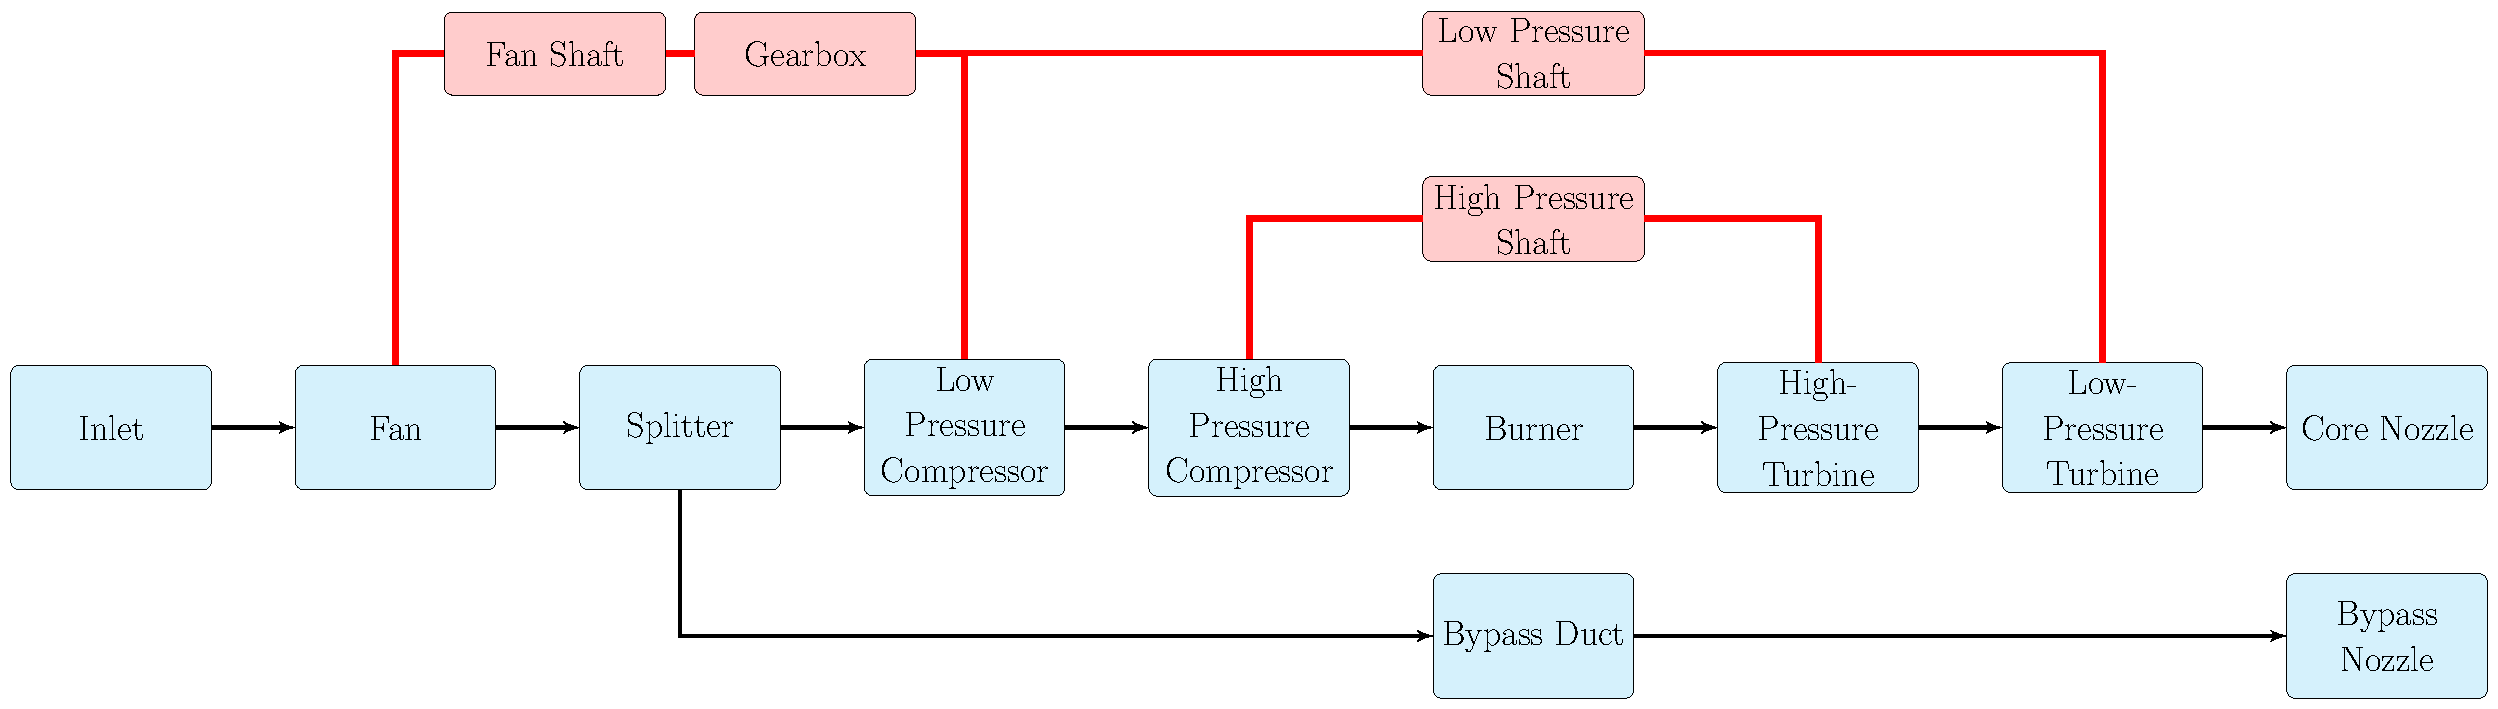
\includegraphics[width=1.0\textwidth]{N3_cycle.pdf}
    \caption{
        Simplified layout of the N+3 engine cycle, adapted from~\citet{Hendricks2019}.
        Black arrows are flow connections, red lines are mechanical connections, blue boxes are cycle elements, red boxes are shaft elements.
        Flow stations are identified with bubble text.
    }
    \label{fig:N3_original}
\end{figure}

\subsection{Water Recovery Model}
We implemented the closed-loop water recovery system as a feedback cycle that extracts water from the exhaust stream and injects it upstream of the HPC.
We chose this injection location following a study by NASA, Boeing, and Rolls-Royce~\cite{Daggett2010} that claims water injection directly into the combustor is unnecessary.
The water vapor recovery component sits downstream of the LPT and extracts water from the flow before exiting the core nozzle.
% [x] TODO: AL-PA, add a sentence about the assumptions for the vapor recovery instead of the mentioning the condenser
We assume that a fraction of the total water available in the exhaust stream is recovered and that there are no pressure or temperature losses associated with this process.
% NOTE: AL-PA, we will talk about the condenser when we discuss the results of the pressure recovery parameter sweep.
The component flow interface and mechanical connections, including the water injector and water extractor, are depicted in Figure~\ref{fig:n3_cycle}.

\begin{figure}[hbt!]
    \centering
    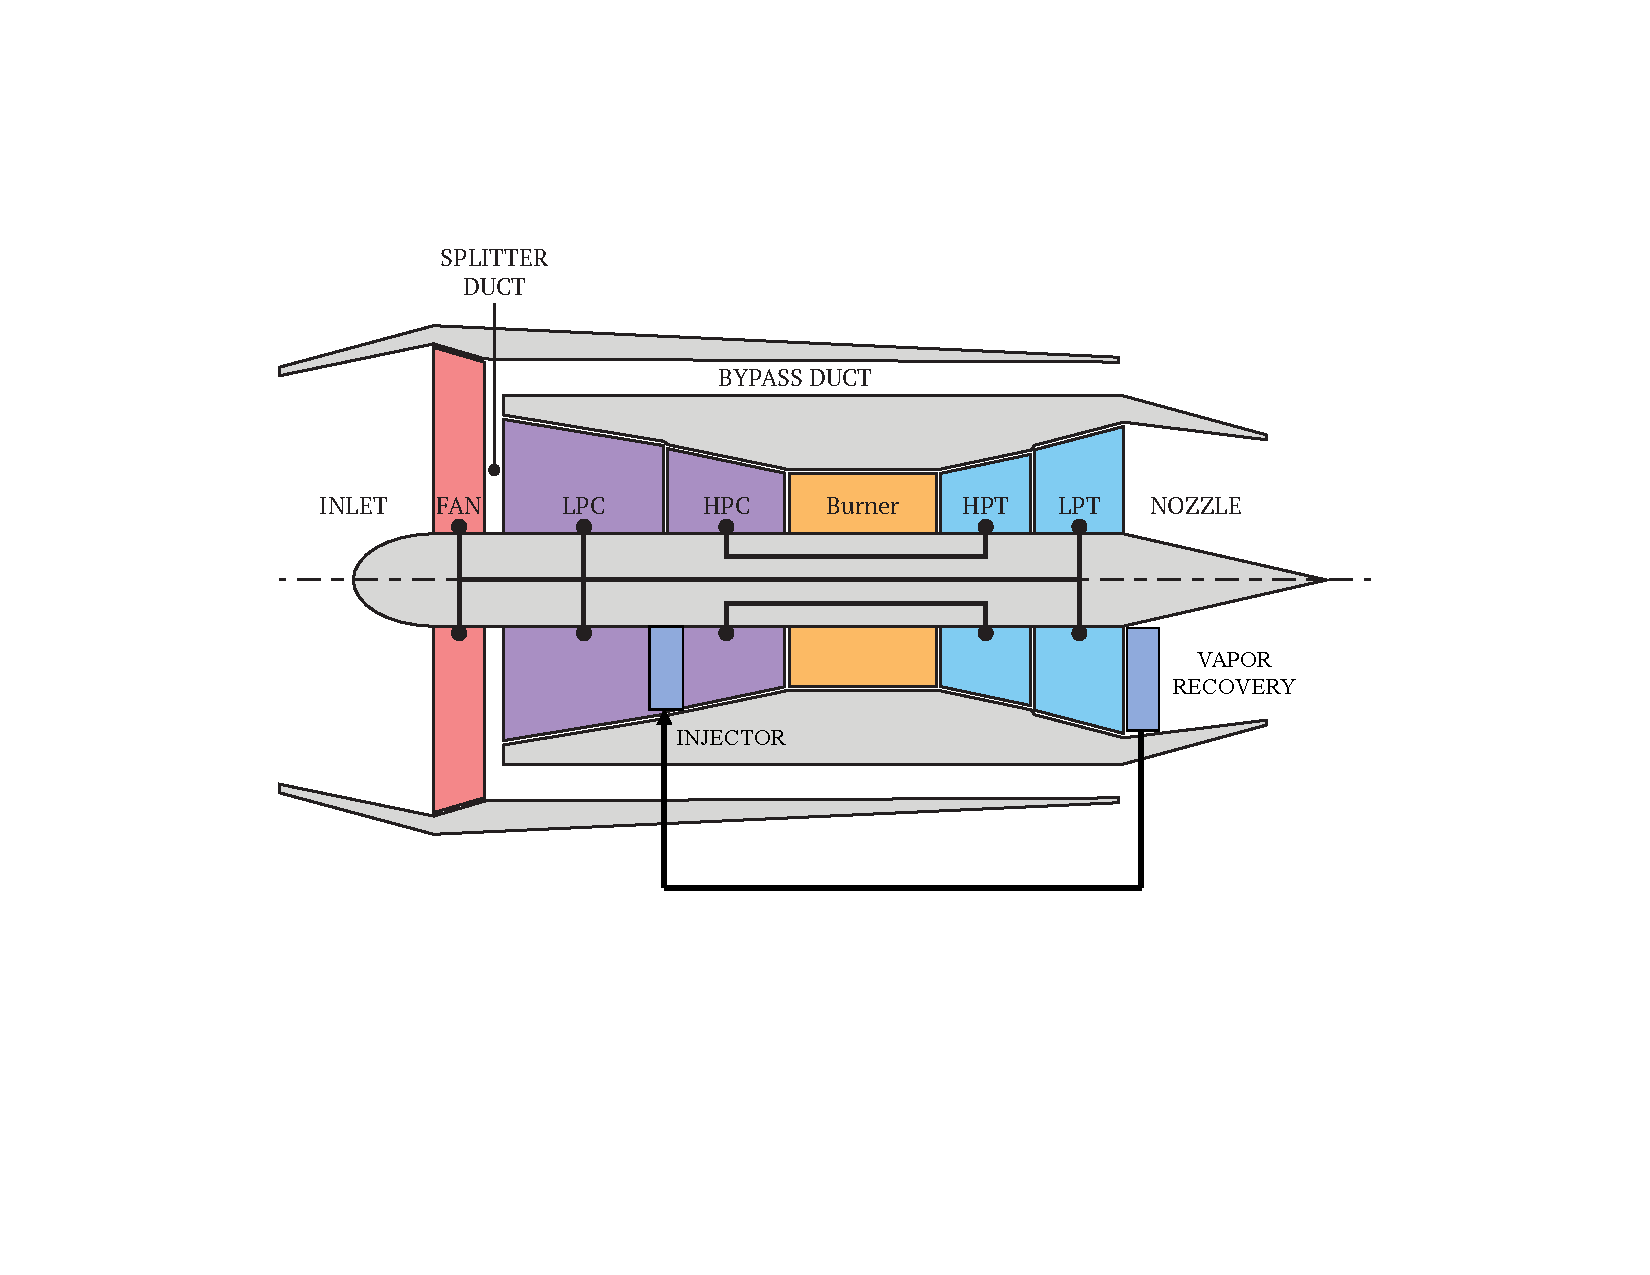
\includegraphics[width=0.75\textwidth]{turbofan_wvr.pdf}
    \caption{
        The configuration of a high-bypass turbofan model with an integrated closed-loop water vapor recovery and injection system.
        The water vapor recovery system (extractor) extracts a fraction of the water in the core stream and re-injects it upstream of the high-pressure compressor.
        This diagram illustrates the feedback effect that this implementation has on the overall core flow.}
    \label{fig:n3_cycle}
\end{figure}

To account for the humidity of the inlet air as well as the increased humidity after water injection, we modified the composition of the air mixture upstream of the combustor.
pyCycle provides a \texttt{wet-air} dataset that introduces \ce{H2O} molecules to the composition of air.
We prescribe atmospheric mass-specific humidity as a water-to-air ratio (WAR) that is defined as the ratio of \ce{H2O} to air in the reactants of the inflow mixture.
% [x] TODO: AL-PA, Reference Table 1 with humidity values as well.
\citet{Kalnay1996} give the humidity values for each flight condition, provided in Table~\ref{tab:flight_conds}.

We introduce two thermodynamic models in pyCycle to capture the effects of water recirculation.
A water injector adds water to the flow upstream of the HPC, while a water extractor diverts a portion of the water in the flow away from the exhaust stream.
The injector operates similarly to fuel injection in the pyCycle combustor component.
We determine a WAR that is analogous to the fuel-to-air (FAR) ratio in the combustor.
This WAR is used to compute the chemical species present in the flow at the current thermodynamic state, determined by the incoming flow.
The new species composition and thermodynamic state are determined using the pyCycle CEA solver~\cite{Gray2017b}.
The water injector inputs are the mass flow rate and mass fraction of water.
We can solve for the mass flow rate on a mixture basis using the WAR, or directly by specifying the mass flow rate of water.
A schematic of the injector is shown in Figure~\ref{fig:injector} where \ce{Y_{\ce{H2O}}} is the mole fraction of water molecules.

% NOTE: AL-PA, I turned this into a subfigure to save some space
\begin{figure}[hbt!]
    \centering
    \begin{subfigure}[t]{0.49\textwidth}
        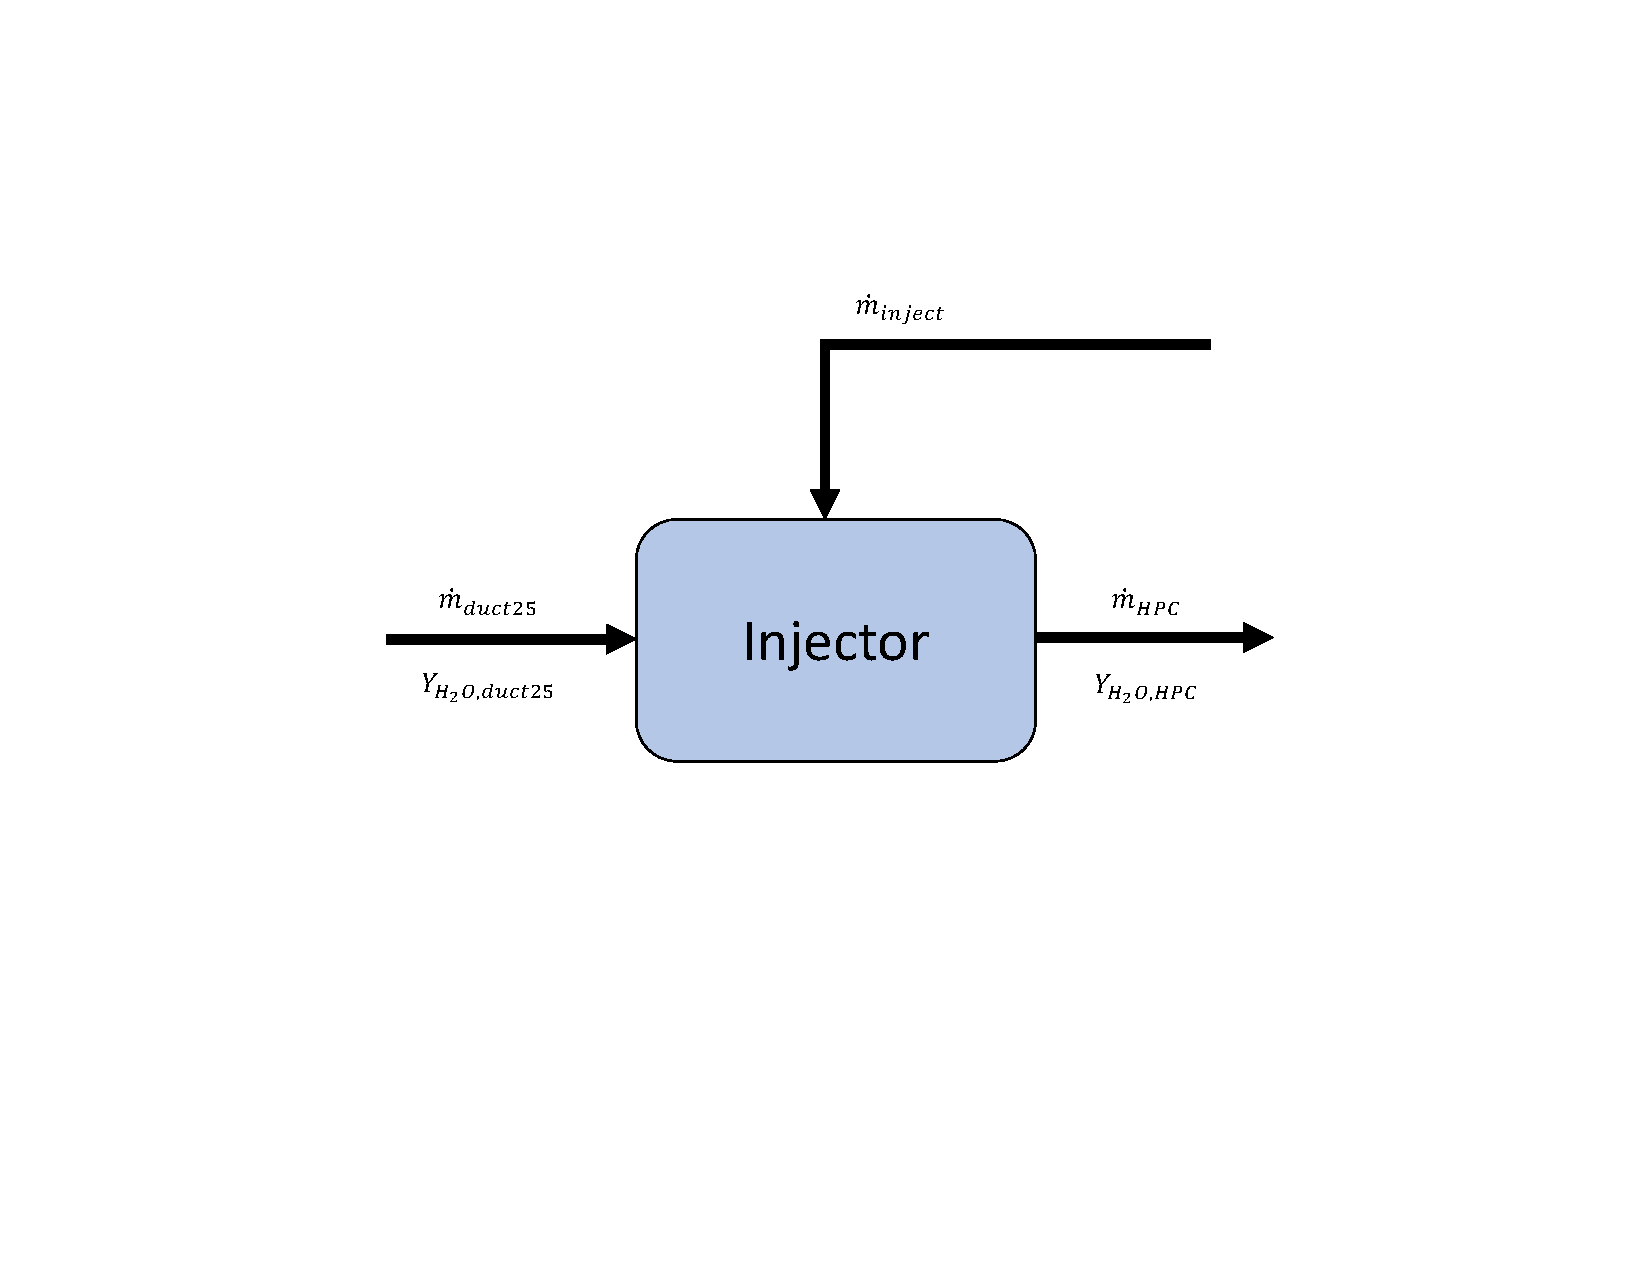
\includegraphics[width=\textwidth]{injector.pdf}
        \caption{
            Water from the extractor is simply injected into the core flow upstream of the high-pressure compressor.
        }
        \label{fig:injector}
    \end{subfigure}
    \hspace{2pt}
    \begin{subfigure}[t]{0.49\textwidth}
        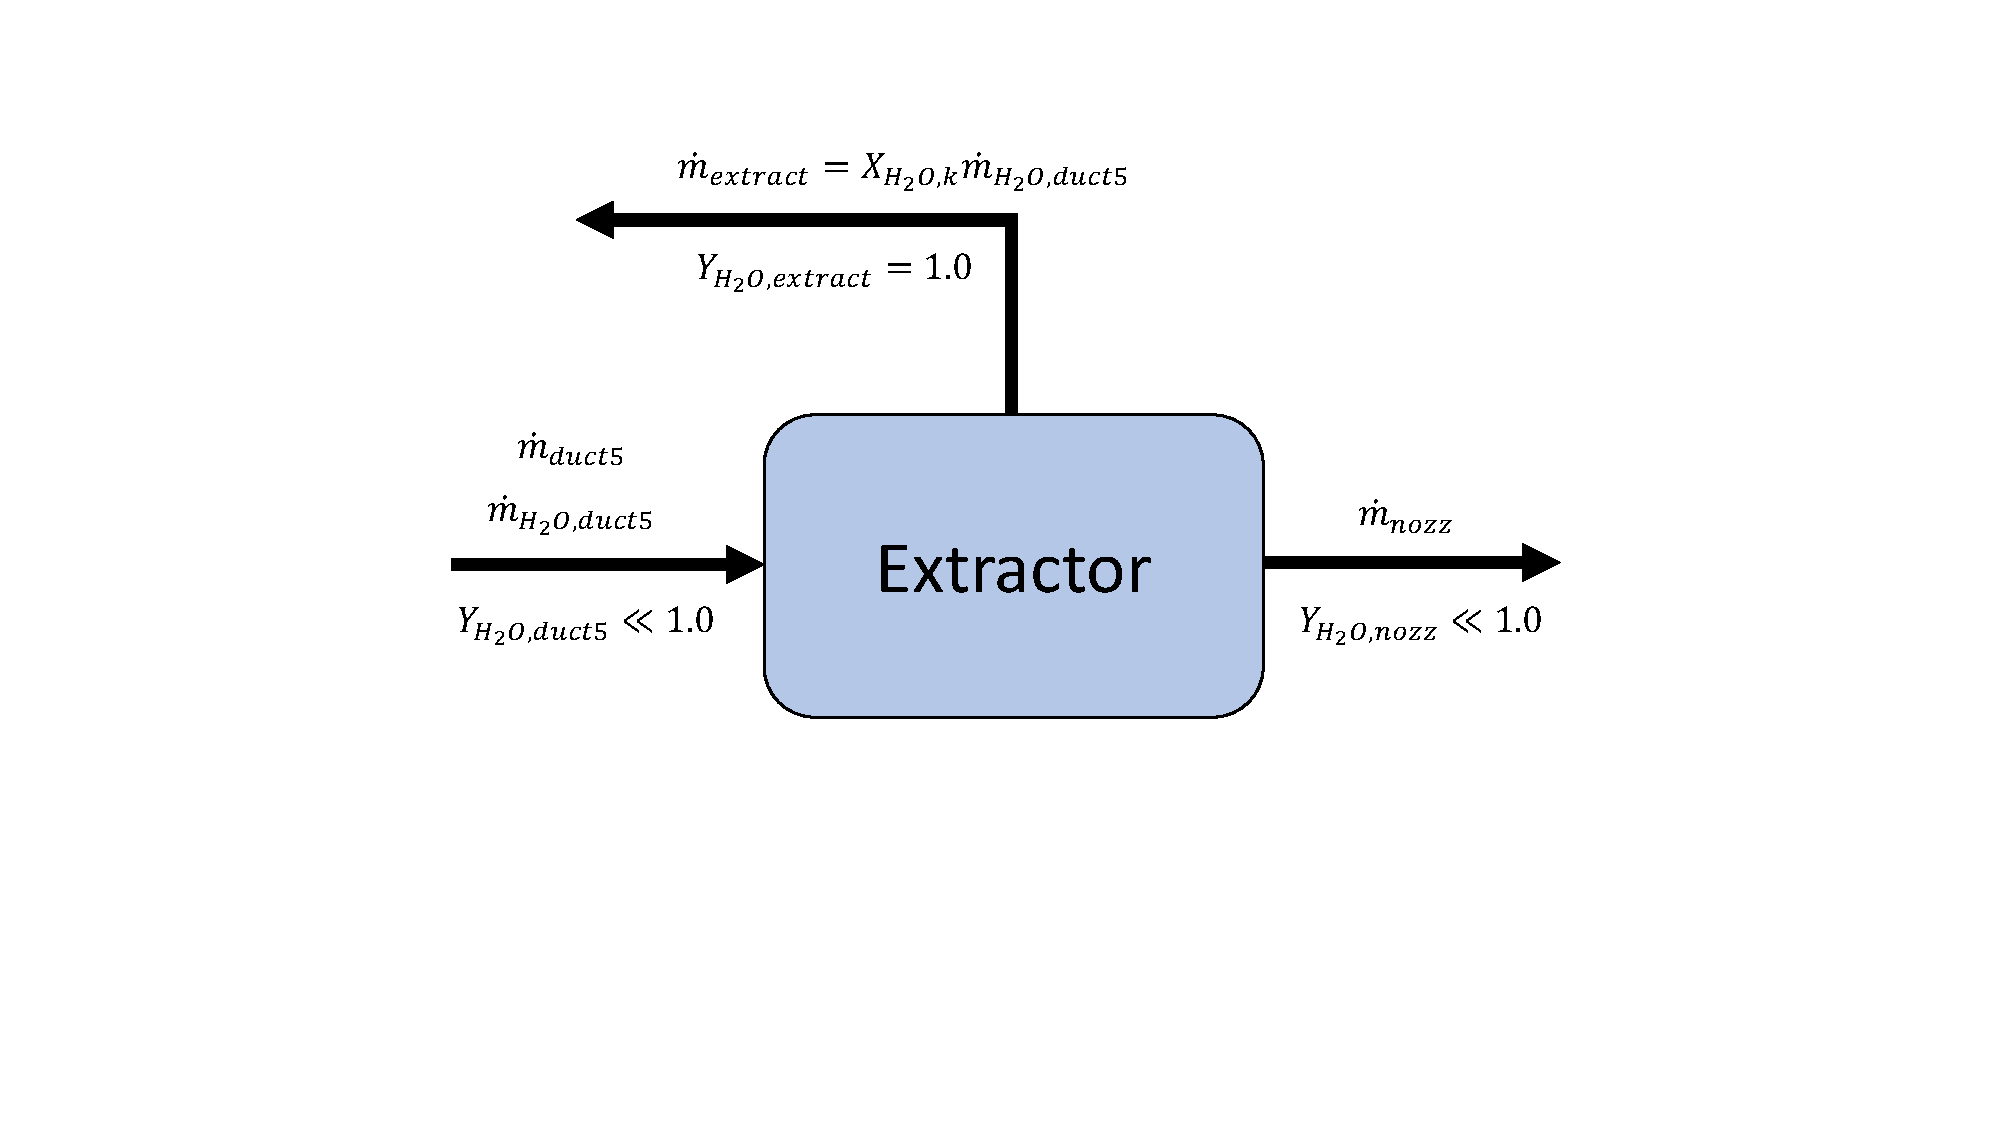
\includegraphics[width=\textwidth]{extractor.pdf}
        \caption{
            We extract a fraction of the mass flow of water determined by the molar composition.
            The extracted water is routed from Duct5 back upstream to the injector and the rest is exhausted out the nozzle.
        }
        \label{fig:extractor}
    \end{subfigure}
    % [x] TODO: AL-PA, Might want to add a bit more to this caption if you think it's necessary.
    \caption{Injector (left) and extractor(right) diagrams that show the inputs and output streams of each component.
        The inputs and outputs show which flow values are used to compute the amount of recirculated water.}
    \label{fig:extract_inject}
\end{figure}

The water extractor model diverts a fraction of a specific species from one flow path to another.
The CEA solver calculates the inflow composition and the extractor separates a specific species based on a mass fraction input.
The composition of the core stream is updated to represent the remaining mixture after the extractor model removes the species from the incoming flow.
We then solve for the thermodynamic state and flow path areas at the outflow of both extractor streams.
A simple schematic of the extractor is shown in Figure~\ref{fig:extractor} where \ce{Y_{\ce{H2O}}} is the mole fraction of water molecules and \ce{X_{\ce{H2O}}} is the mass fraction of water that is recovered from the core stream.
We connect one outflow stream of the extractor to the inflow stream of the injector to complete the water recirculation system.

% NOTE: AL-PA, I made this a new paragraph (no content change)
The model results in a mismatch between the mass flow rate upstream of the HPC and the mass flow rate exiting the core nozzle.
To preserve conservation of mass, we treat the water recirculation as a nonlinear cycle that must converge before the engine calculation is physically balanced.
In this model, we are assuming the water molecules are removed from the exhaust stream with no pressure or temperature losses.
We also assume the injected water molecules are at the same pressure and temperature as the air flow just before the HPC.
% NOTE: AL-PA, I removed this because I don't think the reader will understand the phase-change nuances with 0D cycle and CEA
We illustrate the water recirculation loop and the nonlinear solver connections in Figure~\ref{fig:N3_xdsm_full}.

\begin{figure}[hbt!]
    \centering
    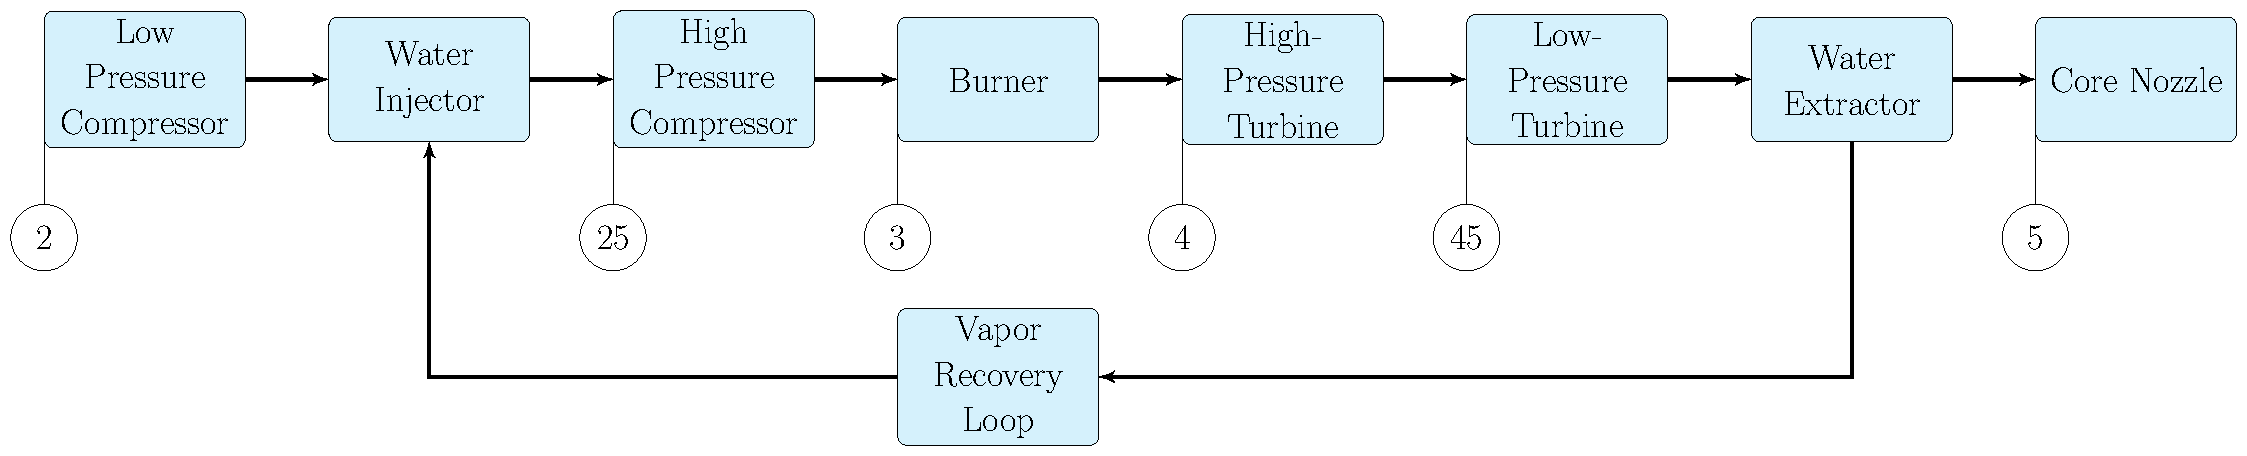
\includegraphics[width=1.0\textwidth]{N3_CLVR_cycle.pdf}
    \caption{
        Simplified layout of the N+3 engine cycle with the closed-loop vapor recovery.
        Black arrows are flow connections, blue boxes are cycle elements.
        Flow stations are identified with bubble text.
    }
    \label{fig:n3_clvr}
\end{figure}

\subsection{Multipoint Propulsion Model}
The N+3 model is a collection of components that combine to form a unified zero-dimensional cycle.
The model consists of twenty-five different elements that define the flow path and the mechanical systems.
Thermodynamic quantities are solved and exchanged using CEA at flow path boundaries represented by black arrows between blue flow path components in Figure~\ref{fig:N3_original}.
The fan, gearbox, low pressure, and high pressure systems are connected by three mechanical shafts depicted in red in Figure~\ref{fig:N3_original}.

% NOTE: AL-PA, this ended up a bit choppy, but I think it's better than before.  If you want to adjust things a bit go ahead.
We impose \emph{balance} equations to satisfy the physical governing equations, conservation laws, and design rules.
Balance relationships are formulated as equations in the form $r(u)=0$ where $r$ is a residual function and $u$ is an implicit state variable.
We use Newton based solvers to find the value of the state variables that drive the set of balance residuals to zero.
\citeauthor{Hendricks2019} provide the extensive set of balance equations with further details on the construction of the nonlinear system for the N+3 model.

% NOTE: AL-PA, I added this blurb to introduce multipoint
We operate the engine cycle in different modes depending on the desired conservation relationships, design rules, and flight conditions.
In ``on-design'' mode, we prescribe cycle inputs such as turbo machinery efficiencies, pressure ratios, and combustion temperatures.
The ``off-design'' mode inherits the flow path areas and turbo machinery map scalars from the ``on-design'' analysis.
This approach is known as multi-design point (MDP)~\cite{Schutte2009} analysis.
MDP analysis simultaneously considers the performance and design requirements at each operation to automatically calculate a feasible design.

The ``on-design'' point is top-of-climb (TOC) with ``off-design'' conditions at rolling takeoff (RTO), sea-level static (SLS), and cruise (CRZ).
% To account for each of these operating conditions, the N+3 model uses a technique called Multipoint Design Point (MDP) modeling to converge the model to an engine design.
Table~\ref{tab:flight_conds} shows the different altitudes and mach numbers for each flight condition.
% We consider these points because they either limit the performance at cruise or present critical design considerations for the propulsion system.
% [x] TODO: AL-PA, Add a small table to show the mach and altitude of each flight condition
\begin{table}[hbt!]
    \centering
    \caption{Altitude and mach numbers at each of the flight conditions considered in the multipoint formulation.
        The humidity ratios were computed from humidity data~\cite{Kalnay1996}.
    }
    \begin{tabular}{l r r r r l}
        \hline
        Parameter      & TOC     & RTO   & SLS   & CRZ     & Units      \\
        \hline
        Altitude       & 35000   & 0     & 0     & 35000   & \si{ft}    \\
        Mach           & 0.8     & 0.25  & 0.0   & 0.8     & -          \\
        Humidity Ratio & 0.00017 & 0.009 & 0.009 & 0.00017 & \si{kg/kg} \\
        \hline
    \end{tabular}
    \label{tab:flight_conds}
\end{table}
% [x] TODO: AL-PA, You should explain why each design point is important in a separate sentence for each.
%   - For example, the SLS point is important for making sure the turbo machinery and flow paths are designed to meet a static thrust target
%   - The RTO point is limiting for temperature, etc...
% [x] TODO: AL-PA, Consider re-writing this section using the comments from the previous TODO.  Be more concise and direct with the language here.
% [x] TODO: AL-PA, This is a big run-on sentence.  Consider breaking it up and being more specific about the requirements at each design point.  See previous comments.
The design rules at SLS ensure that the turbo machinery and flow paths meet the static thrust target.
Rolling takeoff limitations constrain the upper limit of the combustor temperature and subsequently the cooling requirements of the turbines.
The cooling mass flow rates ($\dot{m}_{\rm{cool},k}$) are passed from the RTO point to all other flight conditions creating a cyclic connection.
We add a fuel burn objective at cruise to optimize the engine performance during the longest flight segment.
We size the water recovery system at the CRZ condition because it has the greatest impact on fuel burn over the flight envelope.
Similarly to $\dot{m}_{\rm{cool},k}$, the water recovery mass flow rates ($\dot{m}_{\rm{water},k}$) are connected back to the other operating points.
Figure~\ref{fig:N3_xdsm_full} is an extended design structure matrix (XDSM)~\cite{Lambe2012a} diagram depicting the coupled multipoint model.
The interconnections between flight conditions create a nonlinear cyclic loop with feedback between flight conditions.
The converged model represents a feasible multipoint engine that accounts for design considerations and conservation laws at all four operating conditions.
% [x] TODO: AL-PA, I removed a lot of stuff here to simplify this section.
%                  - Ultimately I think we need to reference the pyCycle paper to prevent duplicating a bunch of math/text
%                  - If you are okay with this check off this TODO.  If not feel free to add a bit more and then check it off.
We direct the reader to the N+3 multipoint model definition in the paper by \citet{Hendricks2019} for the detailed description of the balance relationships.

% [x] TODO: AL-PA, Already discussed, but this should be the only "fine-detail" XDSM in the paper.
% [x] TODO: AL-PA, Make the figure use the entire text width so that it's easier to read.  Might have to reposition a bit.
% [x] TODO: AL-PA, Remove the mdot_inject and mdot_extract stuff, just call it mdot_water
% [x] TODO: AL-PA, copy the format of the cooling flow connections for the water mass flow rates
% [x] TODO: AL-PA, "Area" should be abbreviated to just the letter "A"
% [x] TODO: AL-PA, Change the component types for TOC, RTO, SLS, CRZ, and BALANCE to be implicit groups. They should show up as red polygons.
\begin{figure}[hbt!]
    \centering
    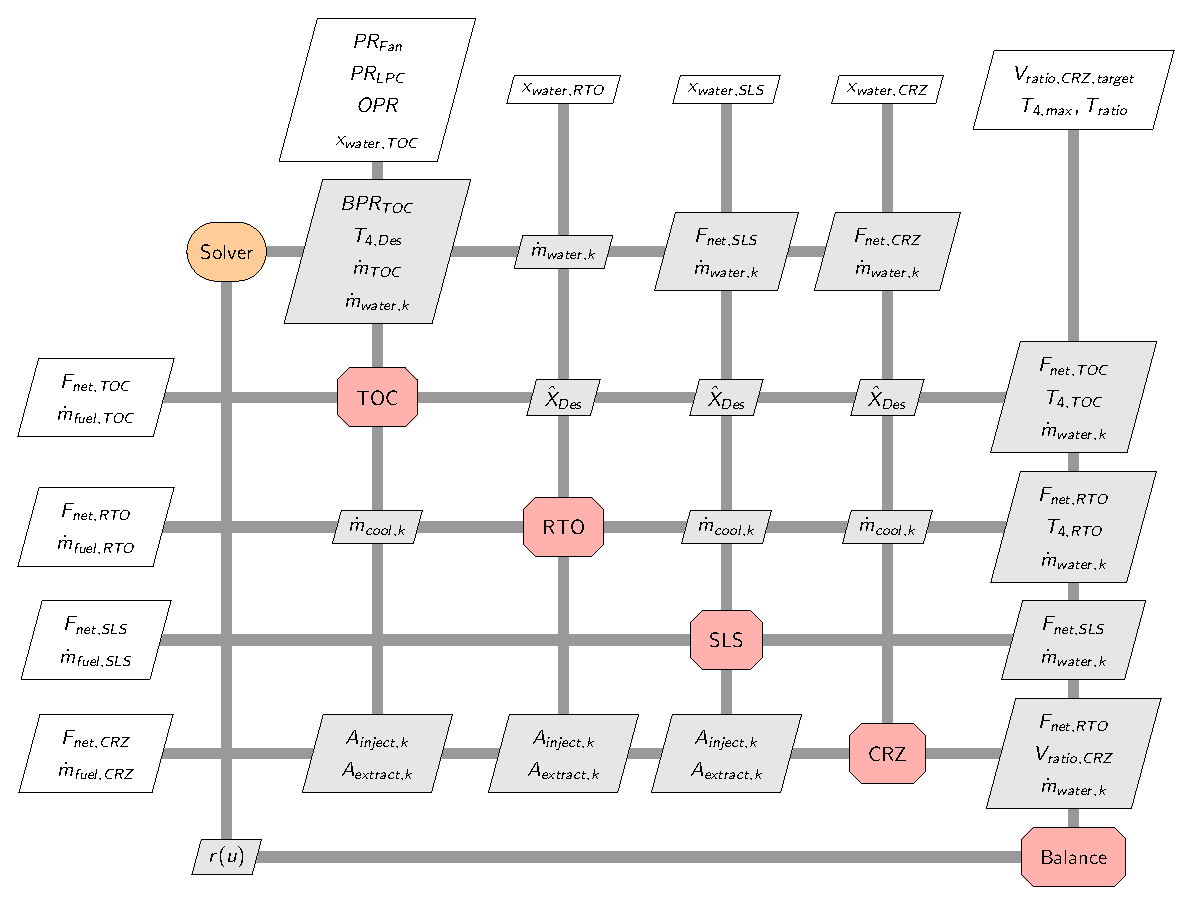
\includegraphics[width=\textwidth]{N3_xdsm_full.pdf}
    \caption{
        Full multidisciplinary design analysis (MDA) model N+3 XDSM diagram.
        This XDSM diagram shows the multipoint coupling between the different operation conditions and shows how the water recovery fractions are used to solve for water mass flow rates.
    }
    \label{fig:N3_xdsm_full}
\end{figure}

\section{Optimization Problem}
\label{sec:optprob}
% NOTE: AL-PA, No reason to have an extra subsection here so I removed it
% \subsection{Problem Statement}
% Briefly discuss the optimization problem
% NOTE: AL-PA, "We will perform" makes it seem like we haven't done the work yet.
We performed MDP gradient-based design optimization of the N+3 engine model considering the TOC, RTO, SLS, and CRZ flight conditions.
% NOTE: AL-PA, I re-wrote this to be more direct
The objective is to minimize fuel burn subject to design and performance constraints.
% [x] TODO: AL-PA, This is a good place to discuss the performance metrics and add the equations for TSEC and explain why it's better for this study than TSFC.
Typical gas-turbine analysis measures the efficiency using the thrust-specific fuel consumption (TSFC).
% For measuring the efficiency of Jet engines, thrust-specific fuel consumption (TSFC) is used in cycle analysis since it represents how much fuel is burned at a given thrust level.
However, this metric is not useful in the comparison of efficiency between Jet-A and hydrogen fueled cycle models because of the differences in fuel density and energy capacity.
% However, when comparing Jet-A and hydrogen fuels this is not such a good metric since a given mass flow rate of hydrogen has an energy content almost 3 times that of Jet-A.
A better metric for comparing Jet-A versus hydrogen is thrust-specific energy consumption (TSEC)~\cite{Adler2023}.
TSEC is TSFC multiplied by the lower heating value (LHV) of the fuel shown in Equation~\eqref{eq:tsec}.

\begin{equation}
    \mathrm{TSFC} = \frac{\dot{m}_{\mathrm{fuel}}}{F_{\mathrm{thrust}}}
    \label{eq:tsfc}
\end{equation}

\begin{equation}
    \mathrm{TSEC} = \frac{\dot{m}_{\mathrm{fuel}} \mathrm{LHV}}{F_{\mathrm{thrust}}} = \mathrm{TSFC} \times \mathrm{LHV}
    \label{eq:tsec}
\end{equation}
% In this work we are concerned with minimizing fuel burn of the engine subject to thrust constraints.
% [x] TODO: AL-PA, TSEC is not the objective.  Fuel burn is the objective.  TSEC is the efficiency metric of interest.
TSEC will be used as a efficiency metric at the cruise condition to compare the two fuels in the results.
% [x] TODO: AL-PA, explain the important aspects of the XDSM in writing before referencing the figure.
The fuel properties used in the engine model are given in~\ref{fuel_props}~\footnote{\url{https://www.smartcockpit.com/docs/Jet_Fuel_Characteristics.pdf}}~\footnote{\url{https://www.engineeringtoolbox.com/fuels-higher-calorific-values-d_169.html}}.

% [x] TODO: AL-PA, Why are some of the fist words in the descriptions capitalized but not others?  I think this should be consistent.
% [x] TODO: AL-PA, Change the lower heating value references to footnotes. i.e \footnote{\url{...}}
\begin{table}[hbt!]
    \centering
    \caption{
        N+3 model fuel properties.
        The lower heating values are given for each fuel used to compute TSEC.}
    \begin{tabular}{r r r l}
        \hline
        Parameter              & Value & Units        & Description                  \\
        \hline
        $\rm{LHV}_{\rm{JetA}}$ & 18564 & \si{BTU/lbm} & Lower heating value of Jet-A \\
        $\rm{LHV}_{\rm{H2}}$   & 51591 & \si{BTU/lbm} & Lower heating value of H2    \\
        \hline
    \end{tabular}
    \label{fuel_props}
\end{table}

We present a high-level summary of the optimization framework using an XDSM diagram in Figure~\ref{fig:N3_opt_xdsm}.
The XDSM diagram shows the design variable, objective, and constraint connections between the optimization algorithm and the multipoint analysis model.
The detailed optimization problem description is provided in Table~\ref{tab:opt_problem}.
% Large multidisciplinary optimization problems are commonly represented with extended design structure matrix (XDSM) diagrams.
% XDSM diagrams are used to visualize the complex implicit and explicit relationships between functions, the solver, and optimizer.
% An XDSM diagram of the optimization problem with the multipoint formulation is shown in Figure~\ref{fig:N3_opt_xdsm}.

% [x] TODO: AL-PA, simplify this XDSM to show just the optimization setup. Condense the MDA into a single block and remove all the multipoint acronyms.
% [x] TODO: AL-PA, Combine the TOC and Off design stack into a single block that just says (MDP Cycle Model)
% [x] TODO: AL-PA, Remove the map scalar, core area, and water recovery area connections
% [x] TODO: AL-PA, The symbol for thrust is "F" not "T"
% [x] TODO: AL-PA, Show the final outputs on the left side of the XDSM and include a superscript "*" to denote optimal values. i.e \dot{m}_\text{fuel}^*
\begin{figure}[!hbt]
    \centering
    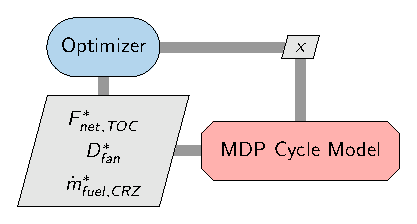
\includegraphics[width=0.5\textwidth]{N3_opt_XDSM.pdf}
    \caption{
        XDSM diagram of the multipoint optimization problem with objective, constraints, and MDA block.
        The XDSM diagram shows the variables and outputs within the optimization model and how each of these values is connected to the optimizer and MDA block.}
    \label{fig:N3_opt_xdsm}
\end{figure}

\begin{table}[hbt!]
    \centering
    \caption{
        Multipoint optimization problem definition.
        The objective function is the fuel flow rate at the cruise condition.
        The constraints are net thrust and engine diameter constraint at the design point, TOC.
    }
    \small
    \renewcommand{\arraystretch}{1.2}
    \begin{tabular}{r l l r l}
        \toprule
                        & Variable/Function              & Description                                                              & Units            & Quantity \\
        \hline
        minimize        & $\dot{m}_{\rm{fuel,CRZ}} $     & Fuel flow rate at CRZ                                                    & \unit{lbm/s}     & 1        \\
                        &                                &                                                                          &                  &          \\
        with respect to & $X_{\rm{H_2O,CRZ}}$            & Water recovery mass fraction at CRZ                                      & -                & 1        \\
                        & $\rm{PR}_{\rm{fan,TOC}}$       & TOC fan pressure ratio                                                   & -                & 1        \\
                        & $\rm{PR}_{\rm{LPC,TOC}}$       & TOC low-pressure compressor pressure ratio                               & -                & 1        \\
                        & $\rm{OPR}_{\rm{TOC}}$          & TOC overall pressure ratio                                               & -                & 1        \\
                        & $T_{4,\rm{RTO}}$               & RTO combustor temperature                                                & \unit{\degree R} & 1        \\
                        & $T_{4,\rm{ratio}}$             & TOC-to-RTO temperature ratio (Equation~\eqref{t4ratio})                  & -                & 1        \\
                        & $V_{\rm{ratio,CRZ}}$           & Core-to-bypass nozzle velocity ratio at CRZ (Equation~\eqref{eq:vratio}) & -                & 1        \\
        \cline{3-5}
                        &                                & Total                                                                    &                  & 7        \\
                        &                                &                                                                          &                  &          \\
        subject to      & $F_{\rm{net,TOC}} \geq 5800.0$ & Target net thrust at TOC                                                 & \unit{lbf}       & 1        \\
                        & $D_{\rm{fan}} \leq 100$        & Maximum Fan Diameter                                                     & \unit{inch^2}    & 1        \\
        \cline{3-5}
                        &                                & Total                                                                    &                  & 2        \\
        \bottomrule
    \end{tabular}
    \label{tab:opt_problem}
\end{table}

% [x] TODO: AL-PA, I would elaborate on this a bit more.  Are these the on-design parameters?  Are they constraints?
% [x] TODO: AL-PA, The N+3 model has a bunch of constraints imposed on the multipoint problem via balance comps.  This is a good place to talk about those.
% [x] TODO: AL-PA, Discuss how using balance comps instead of constraints represents a reduced space problem for the optimizer. (See pycycle paper for more information).
% [x] TODO: AL-AL, I decided this is no longer necessary

% [x] TODO: AL-PA, I would break this up into two or more sentences.
The design variables are specified at different flight conditions.
At the TOC point, we include the fan pressure ratio ($\rm{PR}_{\rm{fan,TOC}}$), LPC pressure ratio ($\rm{PR}_{\rm{LPC,TOC}}$), and overall pressure ratio ($\rm{OPR}_{\rm{TOC}}$).
We add a design variable for maximum turbine inlet temperature at RTO ($T_{4,\rm{RTO}}$).
RTO is the limiting condition for the maximum allowable exit temperature of the burner.
The turbine inlet temperature at TOC is specified by a temperature ratio design variable ($T_{4,\rm{ratio}}$) between the RTO and TOC points, calculated as
% The design variables for this problem are pressure controls such as fan pressure ratio ($\rm{PR}_{\rm{fan,TOC}}$), low pressure compressor pressure ratio ($\rm{PR}_{\rm{LPC,TOC}}$), overall pressure ratio at CRZ ($\rm{OPR}_{\rm{TOC}}$).
% Other design variables are temperature controls such as burner temperature at RTO ($T_{4,\rm{RTO}}$) and the TOC-RTO burner temperature ratio ($T_{4,\rm{ratio}}$).
% TOC-to-RTO burner temperature ratio ($T_{4,\rm{ratio}}$) is shown in Equation~\eqref{t4ratio}.

\begin{equation}
    T_{4,\rm{ratio}} = \frac{T_{4,\rm{TOC}}}{T_{4,\rm{RTO}}}
    \label{t4ratio}
\end{equation}

\noindent
The nozzle velocity ratio at CRZ ($V_{\rm{ratio,CRZ}}$) is also added as a design variable to control the bypass ratio (BPR) at TOC.
The nozzle velocity ratio is defined as

\begin{equation}
    V_{\rm{ratio}} = \frac{V_{\rm{core,ideal}}C_{v,\rm{core}}}{V_{\rm{bypass,ideal}}C_{v,\rm{bypass}}}
    \label{eq:vratio}
\end{equation}
where $V_\text{ideal}$ is the ideal nozzle exit velocity and $C_v$ is the nozzle velocity coefficient that accounts for non-ideal nozzle effects.
The final design variable is the water recovery fraction at CRZ ($X_{\rm{H_2O,CRZ}}$).
% [x] TODO: AL-PA, optimizing for fuel burn subject to net thrust constraint...
% [x] TODO: AL-PA, this isn't the only reason we consider just the water recovery at cruise.  It's also the longest flight segment and contributes the most to long-term performance.
We only include the water recovery fraction at cruise because it has the largest impact on the fuel mass flow rate objective function.
Additionally, the CRZ operating condition is the longest flight segment and contributes the most to long-term engine performance.
The range for each design variable and the associated units are shown in Table~\ref{tab:dv_table}.
% We add the water recovery fraction only at the CRZ point as a design variable since we are optimizing $\dot{m}_{\rm{fuel,CRZ}}$.
\begin{table}[hbt!]
    \centering
    \caption{Design variable ranges for the optimization problem.
    }
    \small
    \renewcommand{\arraystretch}{1.2}
    \begin{tabular}{l l l l}
        Design Variable          & Lower  & Upper  & Units            \\
        \toprule
        $X_{\rm{H_2O,CRZ}}$      & 0.0    & 1.0    & -                \\
        $\rm{PR}_{\rm{fan,TOC}}$ & 1.2    & 1.4    & -                \\
        $\rm{PR}_{\rm{LPC,TOC}}$ & 2.5    & 4.0    & -                \\
        $\rm{OPR}_{\rm{TOC}}$    & 40.0   & 70.0   & -                \\
        $T_{4,\rm{ratio}}$       & 0.5    & 0.95   & -                \\
        $T_{4,RTO}$              & 3000.0 & 3600.0 & \unit{\degree R} \\
        $V_{ratio,CRZ}$          & 1.35   & 1.45   & -                \\
        \bottomrule
    \end{tabular}
    \label{tab:dv_table}
\end{table}
% [x] TODO: AL-PA, You already explained the flight conditions in the multipoint section so not necessary here
% [x] TODO: AL-PA, I would describe the constraints in more detail here.  This might be a good spot to talk about the constraints imposed by the balance comps at the top level.
%                  - i.e the SLS and CRZ net thrust constraints
%                  - i.e how the BPR is set by the nozzle velocity ratio
%                  - i.e The interdependence of the TOC mass flow rate and the RTO temperature
As aforementioned in Section~\ref{sec:method}, the N+3 model uses balance relationships to enforce design, conservation, and performance requirements.
To create a reduced space optimization problem, the N+3 model imposes a set of constraints using additional balance relationships.
These constraints are satisfied using a Newton solver at the analysis level instead of the optimization level.
The advantage of the reduced space approach is that the design is feasible at the completion of each optimization iteration.
\citet{Martins2013} classify this architecture as multidisciplinary design feasible (MDF).
The balance relationships constrain the net thrust at the SLS and CRZ conditions, the BPR at TOC, and the turbine inlet temperature ($T_4$) at RTO.
We summarize the constraints as residuals (r) and the associated implicit states ($\vec{u}$) in Equation~\eqref{eq:balance_cons}.
\begin{equation}
    \label{eq:balance_cons}
    r(\vec{u}) \rightarrow
    \begin{cases}
        \setlength{\tabcolsep}{1pt}
        \begin{tabular}{l l}
            $r(\text{BPR}_\text{TOC})$    & $= (V_\text{ratio,TOC})_\text{des} - V_\text{ratio,TOC} = 0$, \\
            $r(\dot{m}_\text{total,TOC})$ & $= (T_{4,\text{RTO}})_\text{des} - T_{4,\text{RTO}} = 0$,     \\
            $r(\text{FAR}_\text{CRZ})$    & $= 0.9 F_\text{net, TOC} - F_\text{net, CRZ} = 0$,            \\
            $r(\text{FAR}_\text{SLS})$    & $= 1.2553 F_\text{net,RTO} - F_\text{net, SLS} = 0$.          \\
        \end{tabular}
    \end{cases}
\end{equation}

% The net thrust for the SLS and CRZ conditions are set using balance relationships between the RTO and TOC points respectively.
% We prescribe an equality constraint using a balance residual to set the RTO net thrust to \SI{22800}{lbf}.
% Another balance residual constrains the SLS net thrust to be 1.2335 the net thrust at RTO.
% Similarly, the net thrust at CRZ is constrained to be 0.9 times the net thrust at TOC.
% Net thrust for SLS is constrained to be 1.2335 times the net thrust at RTO.
% The bypass ratio (BPR) at TOC is set by the \emph{balance} component such that the CRZ nozzle velocity ratio meets a given target value.
% The CRZ velocity ratio constraint ensures that the core exit velocity is higher than the bypass exit velocity.
% The TOC engine mass flow rate is set by the \emph{balance} component using the combustor temperature at RTO, $T_{4,\rm{RTO}}$.
% [x] TODO: AL-PA, Combine these into a single sentence.

% [x] TODO: AL-PA, Define the T4 ratio with an equation and reference the equation in the table
% [x] TODO: AL-PA, I thought we were only doing recovery fractions at CRZ??
% [x] TODO: AL-PA, Make sure you reference the equations for the DVs/cons in the descriptions so the reader can connect them.
% [x] TODO: PA-PA, explain variable ranges

% Blurb about PyOptSparse and SNOPT
% NOTE: AL-PA, This can all be part of the optimization problem section you don't need a new subsection
% \subsection{Optimization Software}
% NOTE: AL-PA, "pyOptSparse" not "PyOptSparse", i.e the first "p" is not capitalized.
% [x] TODO: AL-AL, need to cite pyOptSparse, SNOPT, and OpenMDAO
% NOTE: AL-PA, I re-wrote most of this to be more concise.
The N+3 pyCycle model is implemented in OpenMDAO~\cite{Gray2019a} to perform multidisciplinary gradient-based optimization with analytic coupled derivatives.
We use pyOptSparse~\cite{Wu2020a} to facilitate the use of state-of-the-art optimization software through a unified python interface.
We solve the optimization problem listed in Table~\ref{tab:opt_problem} with SNOPT~\cite{Gill2005a}, a gradient-based sequential quadratic programming (SQP) algorithm for large-scale constrained problems.
% NOTE: AL-PA, this was confusing and I don't think it add much useful information that the readers will actually understand.

% During initial optimization studies of this model, it was found that when $T_{4,\rm{RTO}}$ and $X_{\rm{H_2O,CRZ}}$ are design variables at the same time they had opposite effects on the design.
% The optimizer increases $X_{\rm{H_2O,CRZ}}$ which allows for a lower optimal $T_{4,\rm{RTO}}$.
% This is likely due to the interdependency between engine mass flow rate and $T_{4,\rm{RTO}}$.
% As the recovery water fraction increases less mass flow rate is required through the engine which lowers the required $T_{4,\rm{RTO}}$ for a required level of thrust.
% It was also observed that $X_{\rm{H_2O,CRZ}}$ is increased until the model breaks due to the CEA solver not being able resolve the increased \ce{H2O} molecules that are injected.
% Since $T_{4,\rm{RTO}}$ would be pushed down to its lower limit, it was set as the optimal value from the optimizations with no water recovery.
% This allowed the optimizer to find the maximum $X_{\rm{H_2O,CRZ}}$ that would allow the most water to be recirculated.
% The upper bound on $X_{\rm{H_2O,CRZ}}$ was found to be around 30\% for Jet-A and 17\% for \ce{H2}.
\section{Results}
\label{sec:results}

\subsection{Optimization Results}
\label{sub:opt_res}
% [x] TODO: AL-PA, I would move the following two lines into the optimization problem section and re-write them to be a single concise sentence.

% [x] TODO: AL-PA, This is confusing.  You have two different optimization problem formulations and that is not clear here.
%                  - I think you need to add information to the previous section about the optimization problem that explains all of this information.
%                    Introducing this at the beginning of the results does not make sense.

% Results of optimization problems
% [x] TODO: AL-PA, Include the optimization and feasibility targets and talk about the number of iterations for each optimization.
% [x] TODO: AL-PA, Add that you are running these optimizations on a laptop and provide a rough estimate for the wall time. i.e "These optimizations run in approximately X number of hours on a laptop"
We performed four optimizations of the N+3 engine cycle.
The optimizations considered Jet-A and hydrogen fuels with and without the water recovery loop.
For the optimizations without water recovery, we removed the water mass fraction design variable in Table~\ref{tab:opt_problem}.
In optimizations with water recovery, we use a constant $T_{4,\text{RTO}}$ from the optimizations without water recovery to aid comparisons between configurations.

The optimality and feasibility targets for the optimizations are both $10^{-6}$.
These optimizations took between 20-30 major SNOPT iterations to reach optimality and were completed in approximately 45 minutes on a standard laptop.
The optimality, feasibility, and merit function for each optimization is shown in Figure \ref{fig:history_summary}.
All four optimization problems converged to the requested feasibility and optimality tolerances.
The optimal design variables for each of the four optimizations are presented in Table~\ref{tab:dv_opt}.
% The merit function reached a final value in about 10 iterations for all cases.
% [x] TODO: AL-PA, No need to explain this and then answer your own observation from the plot.  Just tell the reader what the plot shows.
% [x] TODO: AL-PA, Be cognizant that latex will not always put the figure right above a paragraph.  So saying "From this plot" might not make sense.  Need to directly reference the figure.
% NOTE: AL-PA, The merit function is not a time-dependent quantity, so there's no "steady state".  Its enough to just say the merit function was reduced by X amount in X number of iterations...
% From Figure~\ref{fig:history_summary} we observe quadratic convergence in the optimality of the problem near the optimal solution.

% [x] TODO: AL-PA, Stretch the aspect ratio of this figure and squeeze the height in matplotlib.  You don't need this many values on the y-axis for the summary plots.
% Feasibility, Optimality, Merit history
\begin{figure}[hbt!]
    \centering
    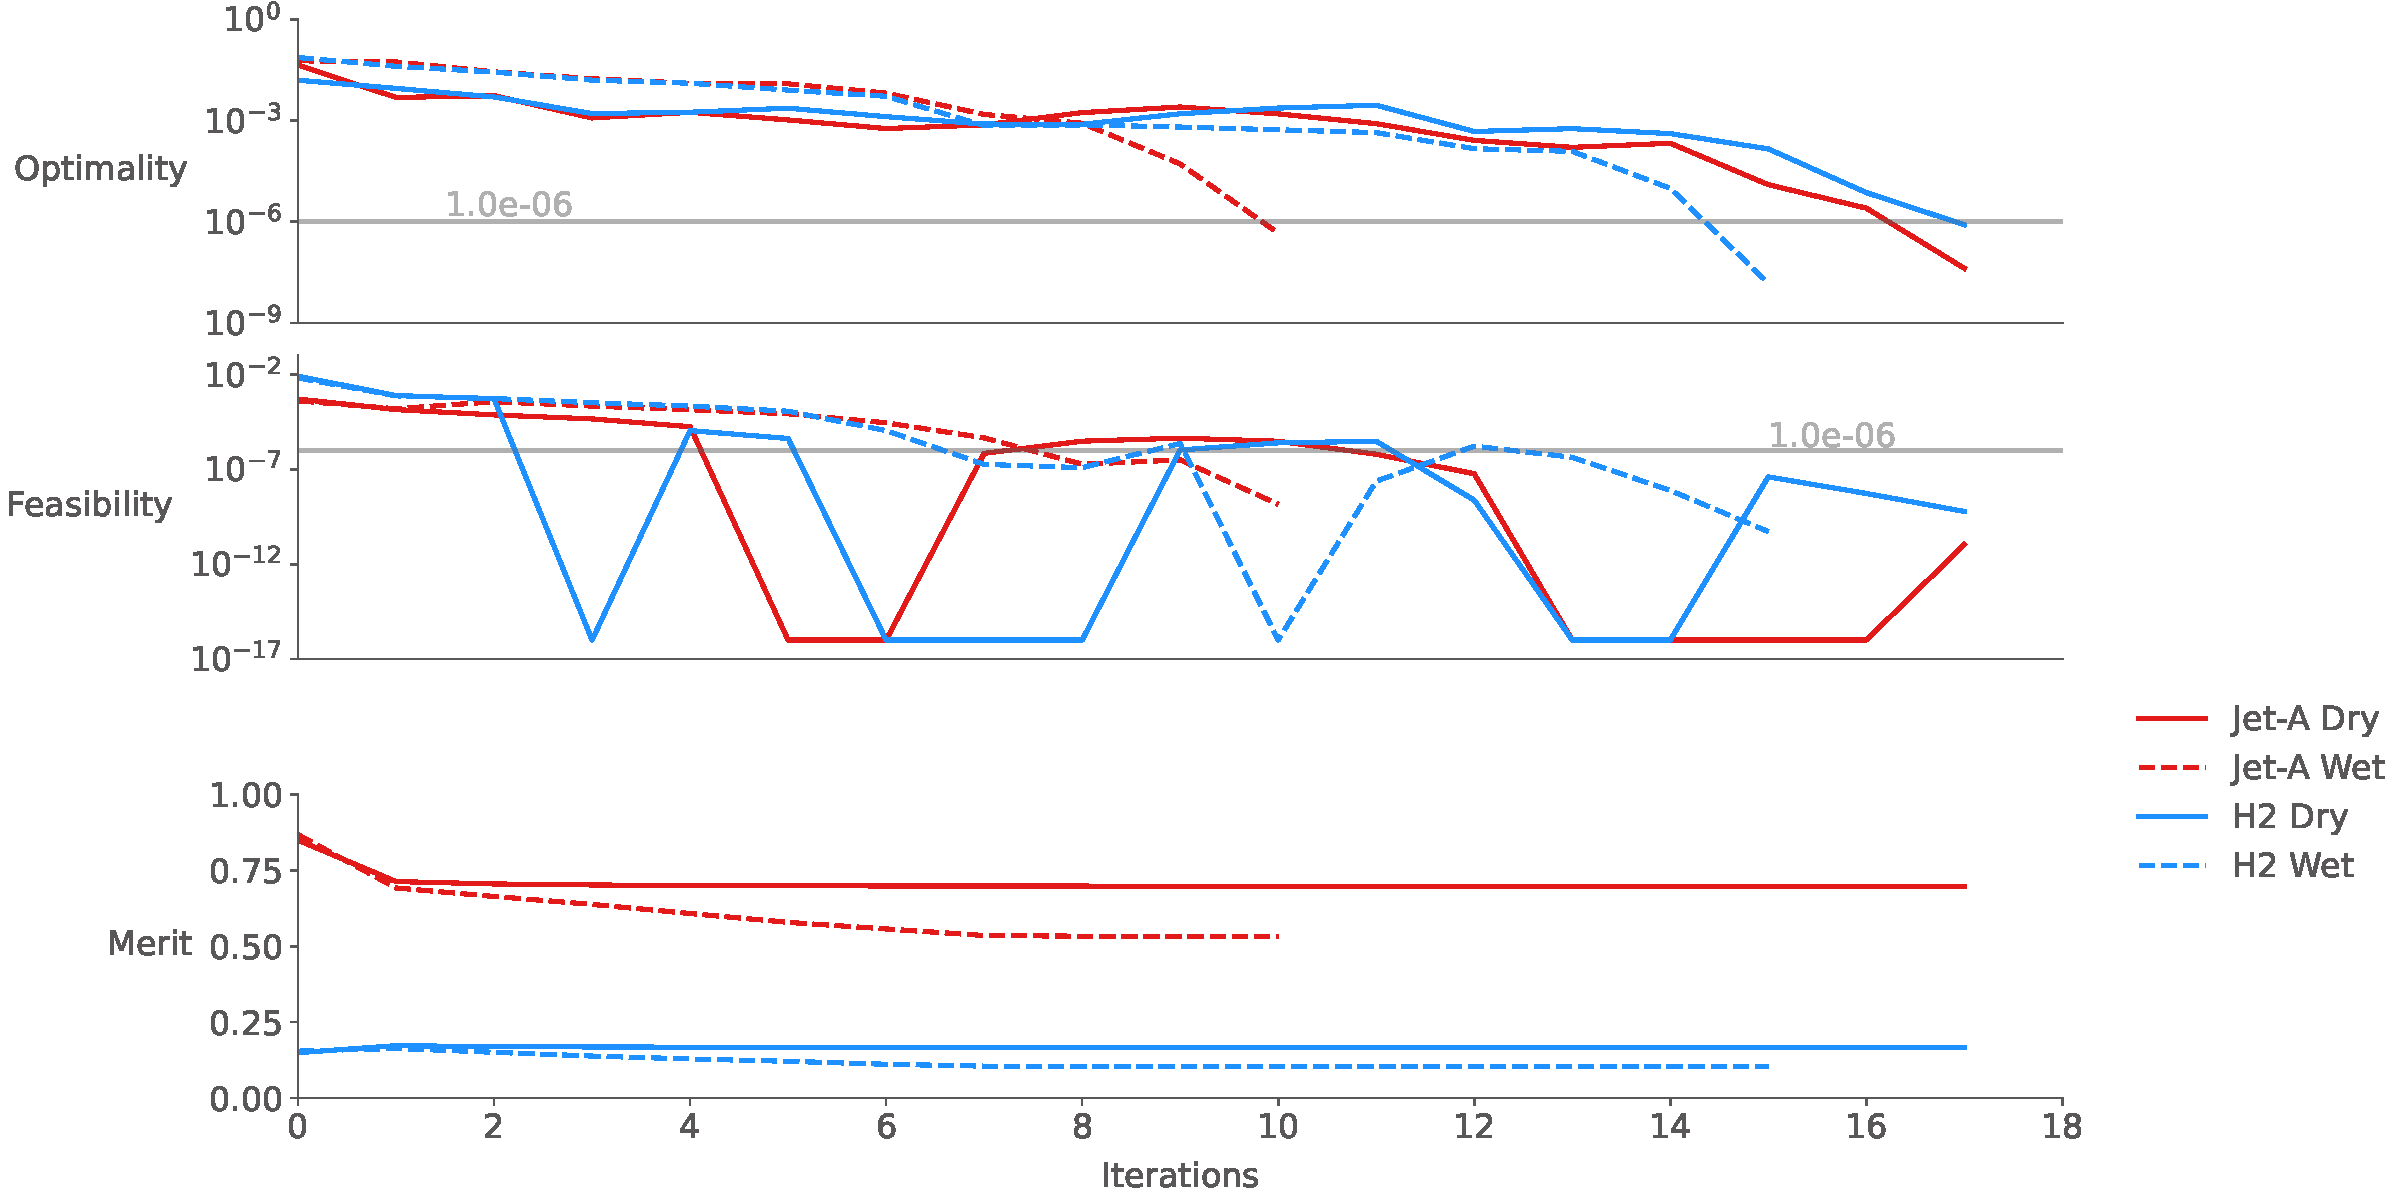
\includegraphics[width=1.0\textwidth]{opt_summary.pdf}
    \caption{The optimality, feasibility, and merit function history for each optimization problem.
        Jet-A without water recovery is shown with the solid lines, the Jet-A with water recovery is shown with dashed lines, hydrogen without water recovery is shown with dash-dot lines, and hydrogen with water recovery is shown with dotted lines.}
    \label{fig:history_summary}
\end{figure}

% [x] TODO: AL-PA, You should explain the plot before it's introduced to the reader.  Stating what's on the figure after it appears doesn't provide any insight.
% [x] TODO: AL-PA, See my previous TODOs but this needs some more explanation in the optimization problem section.
% Note that the $T_{4,\rm{RTO}}$ variables are only present for the optimizations without water recovery and the $X_{\rm{{H_2O},CRZ}}$ variables are present only for the optimizations with water recovery.

\begin{table}[hbt!]
    \centering
    \caption{Optimization results of the N+3 engine for four optimizations using Jet-A and hydrogen fuel with and without water recirculation.
    }
    \small
    \renewcommand{\arraystretch}{1.2}
    \begin{tabular}{r l l l l l l}
                    & Variable/Function         & Jet-A Dry & Jet-A Wet & \ce{H2} Dry & \ce{H2} Wet & Units        \\
        \toprule
        objective   & $\dot{m}_{\rm{fuel,CRZ}}$ & 0.639     & 0.606     & 0.233       & 0.221       & \unit{lbm/s} \\
        % & $\rm{TSEC}_{\rm{CRZ}}$    & 8186.254  & 7766.338  & 8295.236    & 7859.635    & \si{lbm/hr/lbf} \\
        \hline
        variables   & $x_{H2O,CRZ}$             & -         & 0.3       & -           & 0.17        & -            \\
                    & $\rm{PR}_{fan,TOC}$       & 1.285     & 1.292     & 1.288       & 1.297       & -            \\
                    & $\rm{PR}_{LPC,TOC}$       & 4.0       & 4.0       & 4.0         & 4.0         & -            \\
                    & $\rm{OPR}_{\rm{TOC}}$     & 61.012    & 61.188    & 60.660      & 61.952      & -            \\
                    & $T_{4,ratio}$             & 0.913     & 0.911     & 0.918       & 0.915       & -            \\
                    & $T_{4,RTO}$               & 3220.574  & -         & 3204.071    & -           & $^\circ$R    \\
                    & $V_{ratio,CRZ}$           & 1.35      & 1.35      & 1.35        & 1.35        & -            \\
        \hline
        constraints & $F_{net,TOC}$             & 5800.0    & 5800.0    & 5800.0      & 5800.0      & lbf          \\
                    & $D_{Fan}$                 & 100.0     & 100.0     & 100.0       & 100.0       & $in^2$       \\
        \bottomrule
    \end{tabular}
    \label{tab:dv_opt}
\end{table}

% [x] TODO: AL-PA, Constraints are either feasible or they aren't, can't be "for the most part"
% [x] TODO: AL-PA, Elaborate on why we include this parallel axis plot.  Why is it important?  What insight does it provide to the reader?  Compare and contrast the optimization results!
We summarize the optimal values of important thermodynamic variables on a parallel coordinate plot in Figure~\ref{fig:parallel_coords}.
This figure compares the optimal overall design of the N+3 cycle across the four optimization problems.
The TSEC of Jet-A is less than hydrogen with and without water recovery.
However, the TSEC of the optimal cycle with hydrogen combustion and water recovery is less than Jet-A combustion without water recovery.
This suggests that a hydrogen fueled N+3 UHB turbofan with water recovery can compete with the efficiency of a standard Jet-A fueled cycle.
% Figure~\ref{fig:parallel_coords} shows the how each of the optimal overall design of the engine compares across fuel type with and without water recovery.
% [x] TODO: AL-PA, How are they similar? Be specific.
% [x] TODO: AL-PA, I would move a lot of this up to when you introduce the parallel axis plot.
% We see that across the range of values that each optimal value is very similar with the exception of water recovery fraction.

With the addition of water recovery, the propulsive efficiency increases and leads to higher fan pressure ratios and lower TSEC for both fuels.
Additionally, the $T_{4,\text{ratio}}$ is reduced with water recovery leading to cooler combustion temperatures at TOC and subsequently lower fuel burn at CRZ.
We observe the optimal $T_{4,\text{RTO}}$ is larger for Jet-A than hydrogen because hydrogen has a larger combustion flammability limit and the engine can burn at a lower equivalence ratio to attain the same thrust requirements~\cite{Adler2023}.
% [x] TODO: AL-PA, why is this favorable for emissions reduction?  Need to cite or explain.
Burning leaner lowers the FAR which reduces the fuel consumption for a given engine flow rate and is favorable for emissions reduction.
% The additional water in the combustion improves the propulsive efficiency and enables the increase in overall pressure ratio.
% As noted earlier, the water recovery fractions are different because the optimizer pushes $X_{\rm{{H_2O},CRZ}}$ to the highest value it can attain.
% The $\rm{PR}_{fan,TOC}$ and $V_{ratio,CRZ}$ design variables go to their upper and lower limits, respectively.
$V_\text{ratio,CRZ}$ is at the lower bound for all four cases to maximize the amount of mass flow through the bypass stream.

% NOTE: PA-PA/AL replace this with a parallel axis plot?
% [x] TODO: AL-PA, Yeah let's do the parallel axis plot for the basic thermodynamic parameters
% AL-PA, We can make another plot for the water fractions and the dpQp study.
% [x] TODO: AL-PA, Can you make the y-axis range for T4_ratio smaller so we can see the differences a bit better.  Maybe like 0.85 - 0.95
% [x] TODO: AL-PA, Same comment as above but for FPR, maybe 1.28-1.32
% [x] TODO: AL-PA, If a variable has bounds, can we make the y-axis limits match the bounds?
\begin{figure}[hbt!]
    \centering
    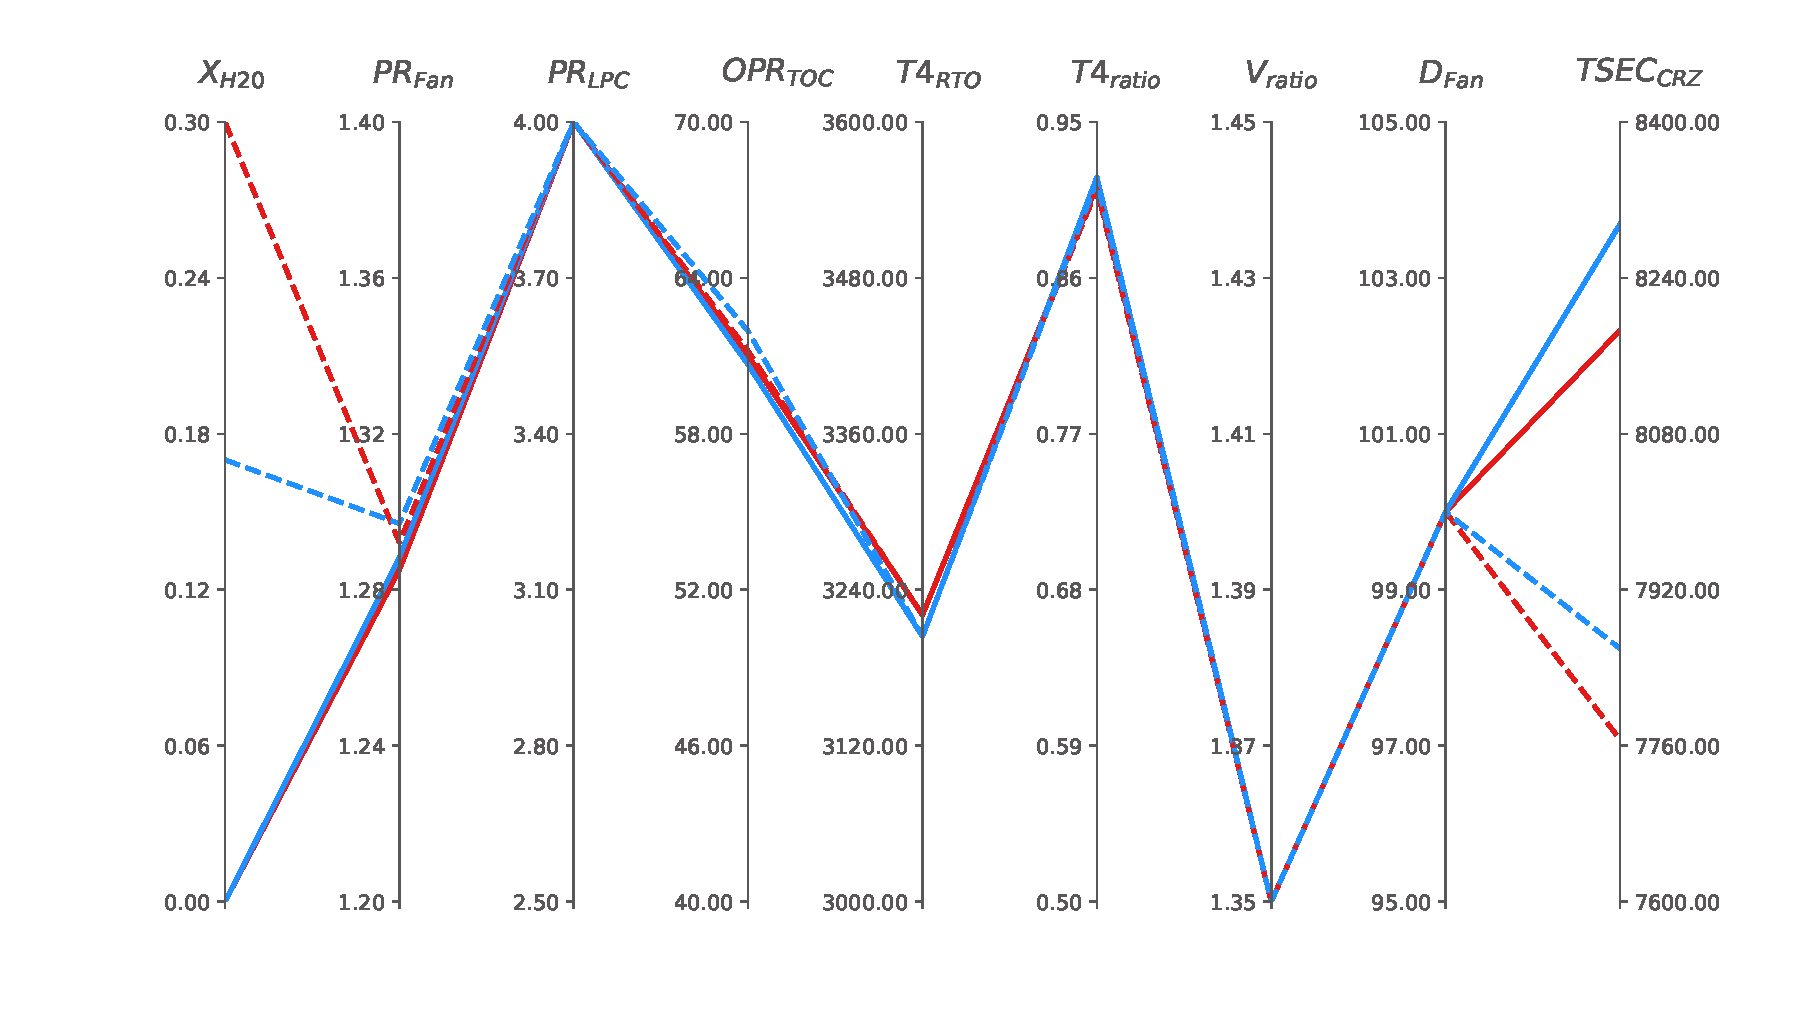
\includegraphics[width=1.0\textwidth]{N3_parallel_coords.pdf}
    \caption{Optimization results of the N+3 engine with and without no water recovery using Jet-A and H2 as the fuel.
        The red lines show Jet-A fuel and the blue lines show \ce{H2} fuel.
        The solid lines show the engine without water recovery and the dashed lines show the engine with water recovery.}
    \label{fig:parallel_coords}
\end{figure}


% [x] TODO: AL-PA, How are the pressure ratios and temperatures different?  Which optimizations resulted in different values?
% $\rm{PR}_{fan,TOC}$ likely goes to its upper value since its more efficient to increase $\rm{PR}_{fan,TOC}$ than $\rm{OPR}_{\rm{TOC}}$.
% The main differences in the engine designs are the pressure ratios and temperatures.
% [x] TODO: AL-PA, Why is pushed to the upper limit?  Explain how it improves the combustion characteristics.
% Between the two fuel types, the water recovery fraction for both is pushed up to the upper limit of the design space.
% One reason the water recovery fraction increases to its upper bound use to improve combustion characteristics of the core flow when fuel is injected.
% The same thrust output can be achieved with water recovery at a lower FAR, slightly lower temperature, and less total mass flow rate.
% The recovery fraction does not directly relate to the mass flow rate of recirculated water since more available water will increase the recirculation flow rate.
% It is noted that recovery fraction for \ce{H2} is smaller than the recovery fraction for Jet-A because there is more water produced in the combustion process.
% However, the mass flow rate of water is larger for \ce{H2} at \SI{0.405}{lbm/s} as opposed to \SI{0.324}{lbm/s} for Jet-A.
% The \ce{H2} fuel has the benefit of recovering more water at a lower fraction of the overall water in the core exhaust.
% We see slightly higher pressure ratios across the fan with water recovery leading to a larger overall pressure ratio.
% [x] TODO: AL-PA, I'm beating a dead horse here but you don't need to say this if you mention it earlier
% [x] TODO: AL-PA, Why is the T4 ratio higher?  Explain it in terms of the fuel properties.  The reader can look at the plot themselves and see that it's higher.
% The $T_{4,\rm{RTO}}$ value for Jet-A is slightly higher than that of \ce{H2}.
% This is most likely due to the combustion properties of \ce{H2} compared to Jet-A.
% \ce{H2} can has a wider combustion flammability limit and allows the engine to burn at a lower equivalence ratio to attain the same thrust requirements.
% Burning leaner not only cools the engine but also reduces fuel consumption.
% [x] TODO: AL-PA, Why are the temperatures colder with the H2 fuel?  Why does water recovery make them even lower?
% [x] TODO: AL-PA, I wouldn't say "cooler" I would say "less than" or "colder"
% Therefore, TOC temperatures are colder with the \ce{H2} fuel and even slightly colder when adding water recovery.
% The engine is likely able to size the components with water recovery so that the same thrust is generated at a lower fuel-to-air ratio.
% Furthermore, adding water recovery at CRZ slightly decreases the $T_{4,\rm{ratio}}$ value.
% As noted earlier, the water recovery and injection allows the engine achieve the same level of thrust at a lower temperature.
% [x] TODO: AL-PA, Why did the optimizer push the value of T4 down with water recovery?  Dig into this more.
% In terms of pressure ratios we see that the fan pressure ratio increases with hydrogen fuel and even more with water recovery.
% This is again likely due to using \ce{H2} and water recovery each resizing the engine to increase the amount of thrust generated by the fan.
% [x] TODO: AL-PA, We want to discuss how the thrust from the fan/core changes when we introduce water recovery.
% NOTE: AL-PA, The idea here is to communicate the effect of water recovery on the core power vs. the fan power.
% We analyzed the gross thrust split between the core and bypass streams of the optimized engine cycles.
% Table~\ref{tab:thrust} shows the breakdown between the two flow paths as percentages of the total gross thrust.
% The breakdown of the gross thrust fractions from the core and bypass nozzles for each point is shown in Table~\ref{tab:thrust}.
% The fraction of gross thrust generated by the core nozzle decreases when we use \ce{H2} and decreases further when adding water recovery.

% Increasing the thrust produced in the bypass stream improves the propulsive efficiency.
% Utilizing the fan more than the core nozzle increases the efficiency of the engine since we are not burning as much fuel but is limited by the maximum size of the fan.
% The increase in $\rm{OPR}_{\rm{TOC}}$ mostly reflects the increase in $\rm{PR}_{fan,TOC}$ and resizes of the turbojet section of the engine with water recovery.
% Additionally, the FAR of the engines with water recovery increases due to a decrease in overall and core mass flow.
% An increase in FAR likely requires a larger OPR to maintain the required thrust while minimizing fuel burn.

% Thrust splits
% [x] TODO: PA-PA: Add thrust splits for each opt
% [x] TODO: AL-PA: I think this should be showing gross thrust from the fan divided by gross thrust from the core.
%                  The idea here is to show percentages of thrust generated by fan/core and how that changes with water recovery.
% \begin{table}[hbt!]
%   \centering
%   \caption{Thrust breakdown for each flight operating condition.
%     The net thrust, gross thrust, and ram drag are shown for each optimization result.
%   }
%   \small
%   \renewcommand{\arraystretch}{1.2}
%   \begin{tabular}{r l l l l l}
%     Point & Thrust Fraction & Jet-A Dry & Jet-A Wet & H2 Dry  & H2 Wet  \\
%     \toprule
%     TOC   & Core            & 6.47\%    & 6.05\%    & 5.95\%  & 5.47\%  \\
%           & Bypass          & 93.53\%   & 93.95\%   & 94.05\% & 94.53\% \\
%     \hline
%     RTO   & Core            & 6.31\%    & 5.87\%    & 5.77\%  & 5.26\%  \\
%           & Bypass          & 93.69\%   & 94.13\%   & 94.23\% & 94.74\% \\
%     \hline
%     SLS   & Core            & 6.11\%    & 5.68\%    & 5.58\%  & 5.09\%  \\
%           & Bypass          & 93.89\%   & 94.32\%   & 94.42\% & 94.91\% \\
%     \hline
%     CRZ   & Core            & 6.02\%    & 5.42\%    & 5.53\%  & 4.71\%  \\
%           & Bypass          & 93.98\%   & 94.58\%   & 94.47\% & 95.29\% \\
%     \bottomrule
%   \end{tabular}
%   \label{tab:thrust}
% \end{table}

% [x] TODO: AL-PA, Again, this table might not be directly above this text in the PDF so you need to use \ref{tab:thrust}.
% [x] TODO: AL-PA, You already showed the constraint values and that the design is feasible, the reader knows what the net thrust should be from that information.
% [x] TODO: AL-PA, Thrust differences?  These values change with mass flow rate which we know is affected by water recovery.  Probably need to remove the following stuff discussing this.
% NOTE: AL-PA, I think you misunderstood what happens in the ram drag/gross thrust calculations.  They are just simple control volume thrust equations.
%              If your mass flow rate changes with water recirculation these will change, but that is expected and not super informative in terms of a comparison.


% [x] TODO: I would change this to the horizontal bar chart and plot both H2 and Jet-A on the same axis
% See this example in niceplots: https://github.com/mdolab/niceplots/blob/main/examples/plot_bar_chart.py and https://github.com/mdolab/niceplots/blob/main/examples/ref/bar_chart.png
% [x] TODO: Can you add a line to bar chart that shows the improvement between baseline Jet-A and hydrogen with water recovery?
\begin{figure}[hbt!]
    \centering
    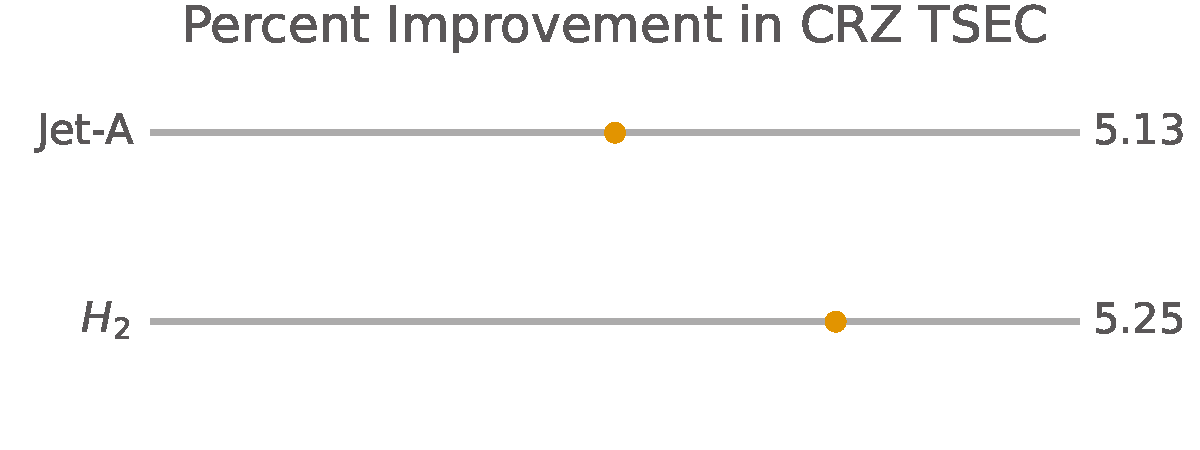
\includegraphics[width=0.65\textwidth]{bar_chart.pdf}
    \caption{Percent relative improvement in thrust specific energy consumption (TSEC) of the N+3 engine with water recovery.
        This plot compares the relative improvement of the two optimization problems with water recovery compared to the optimization problems without water recovery.}
    \label{fig:barchart}
\end{figure}

The TSEC improvement at CRZ due to water recovery for both fuels is shown on a bar chart in Figure~\ref{fig:barchart}.
Water recovery improves the TSEC approximately 5\% for both Jet-A and hydrogen fueled cycles.
% We see an improvement greater than 5\% at CRZ for TSEC for both fuels.
% [x] TODO: AL-PA, This is a good point, but maybe combine with the paragraph after the figure?
Most of the design variables for the optimal designs with and without water recovery vary only slightly for both fuels.
This suggests that the water recovery system accounts for a majority of the efficiency improvements.
Achieving a 5\% reduction in TSEC represents a large fuel savings over the lifecycle of an engine.
% This level of improvement would have a significant reduction in fuel costs over the course of an engine's lifecycle.
% [x] TODO: AL-PA, Add a sentence that introduces this citation and paraphrases the claim.  Then relate it to your findings.
As~\citeauthor{Strom2002} point out, a hydrogen-fueled engine would have close to 3 times more water in the exhaust than a similar Jet-A fueled counterpart.
% [x] TODO: AL-PA, I think we need to add some numbers here for the mass flow rate of water for jet-a and hydrogen to help this claim.
The optimal designs with water recovery have approximately \SI{2.38}{lbm/s} and \SI{1.08}{lbm/s} of water in the core stream for hydrogen and Jet-A, respectively.
% Therefore, \ce{H2} is a much more appealing fuel to use with the proposed closed-loop water recovery system.
Hydrogen combustion offers an immediate reduction in emissions and produces more water in the exhaust stream.
With an advanced water recovery system, we can achieve better TSEC with hydrogen fuel than a standard Jet-A engine without water recovery.
To make hydrogen fueled engines a reality, we need to take advantage of the additional benefits of hydrogen combustion.
\subsection{Condenser Design Space Study}
\label{sub:dpqp_sweep}
% [x] TODO: AL-PA, I would emphasize that we did this sweep to explore the design space following our optimization results.
%                  Might be worth moving this into a new subsection.
% [x] TODO: AL-PA, This study wasn't motivated by a lack of literature, we want to explore the potential design space for the technology we just proposed and analyzed.
The efficiency improvement due to water recirculation warrants a design space study for potential condenser technology.
Companies that are developing engines with water recirculation suggest that hydrogen can be used to as the heat sink for a water condenser~\cite{arpa-e_2021}.
We consider a condenser designed to fit inside the exhaust stream of a hydrogen-fueled turbofan engine.
The trade space for a condenser in the exhaust stream depends on the pressure loss and water recovery capability.
% A low pressure loss condenser would need to be developed for the water recirculation loop to be implemented.
% [x] TODO: AL-PA, dPqP is the relative total pressure loss not just a "pressure loss"

We model the pressure loss across the condenser by varying the relative total pressure loss across Duct5 just upstream of the core nozzle.
% pyCycle handles pressure losses in ducts by specifying a pressure loss coefficient, dPqP.
This pressure loss coefficient (dPqP) is the difference in total pressure across the duct divided by the total pressure at the duct inlet.
% [x] TODO: AL-PA, Try rewording to: "We varied the total pressure loss across the extraction model to simulate drag from an increasingly larger condenser"
% [x] TODO: AL-PA, Elaborate on why we re-optimized the design.  It is because we want to see how the optimal amount of water recovery changes based on the drag incurred by the condenser.
We varied the total pressure loss across the duct to simulate an increasingly larger condenser jutting out into the duct.
We ran an optimization to minimize fuel mass flow rate of hydrogen at each pressure loss value using the formulation for water recovery in Table~\ref{tab:opt_problem}.
% The rest of the engine design variables were optimized during this pressure loss sweep to determine the how the optimal amount of water recovery changed based on drag losses from the condenser.
Figure~\ref{fig:dpqp_sweep} shows the $\rm{TSEC}_{\rm{CRZ}}$ of the optimal engine cycles plotted against dPqP.
The red horizontal line is the $\text{TSEC}_\text{CRZ}$ value of the optimized engine with no water recovery.
The blue region represents the feasible space for potential condenser technology.
\begin{figure}[hbt!]
    \centering
    \begin{subfigure}[t]{0.49\textwidth}
        % [x] TODO: AL-PA, I don't think its benefit vs no-benefit.  The message here is that the blue region is the design space where we can potentially design condenser.
        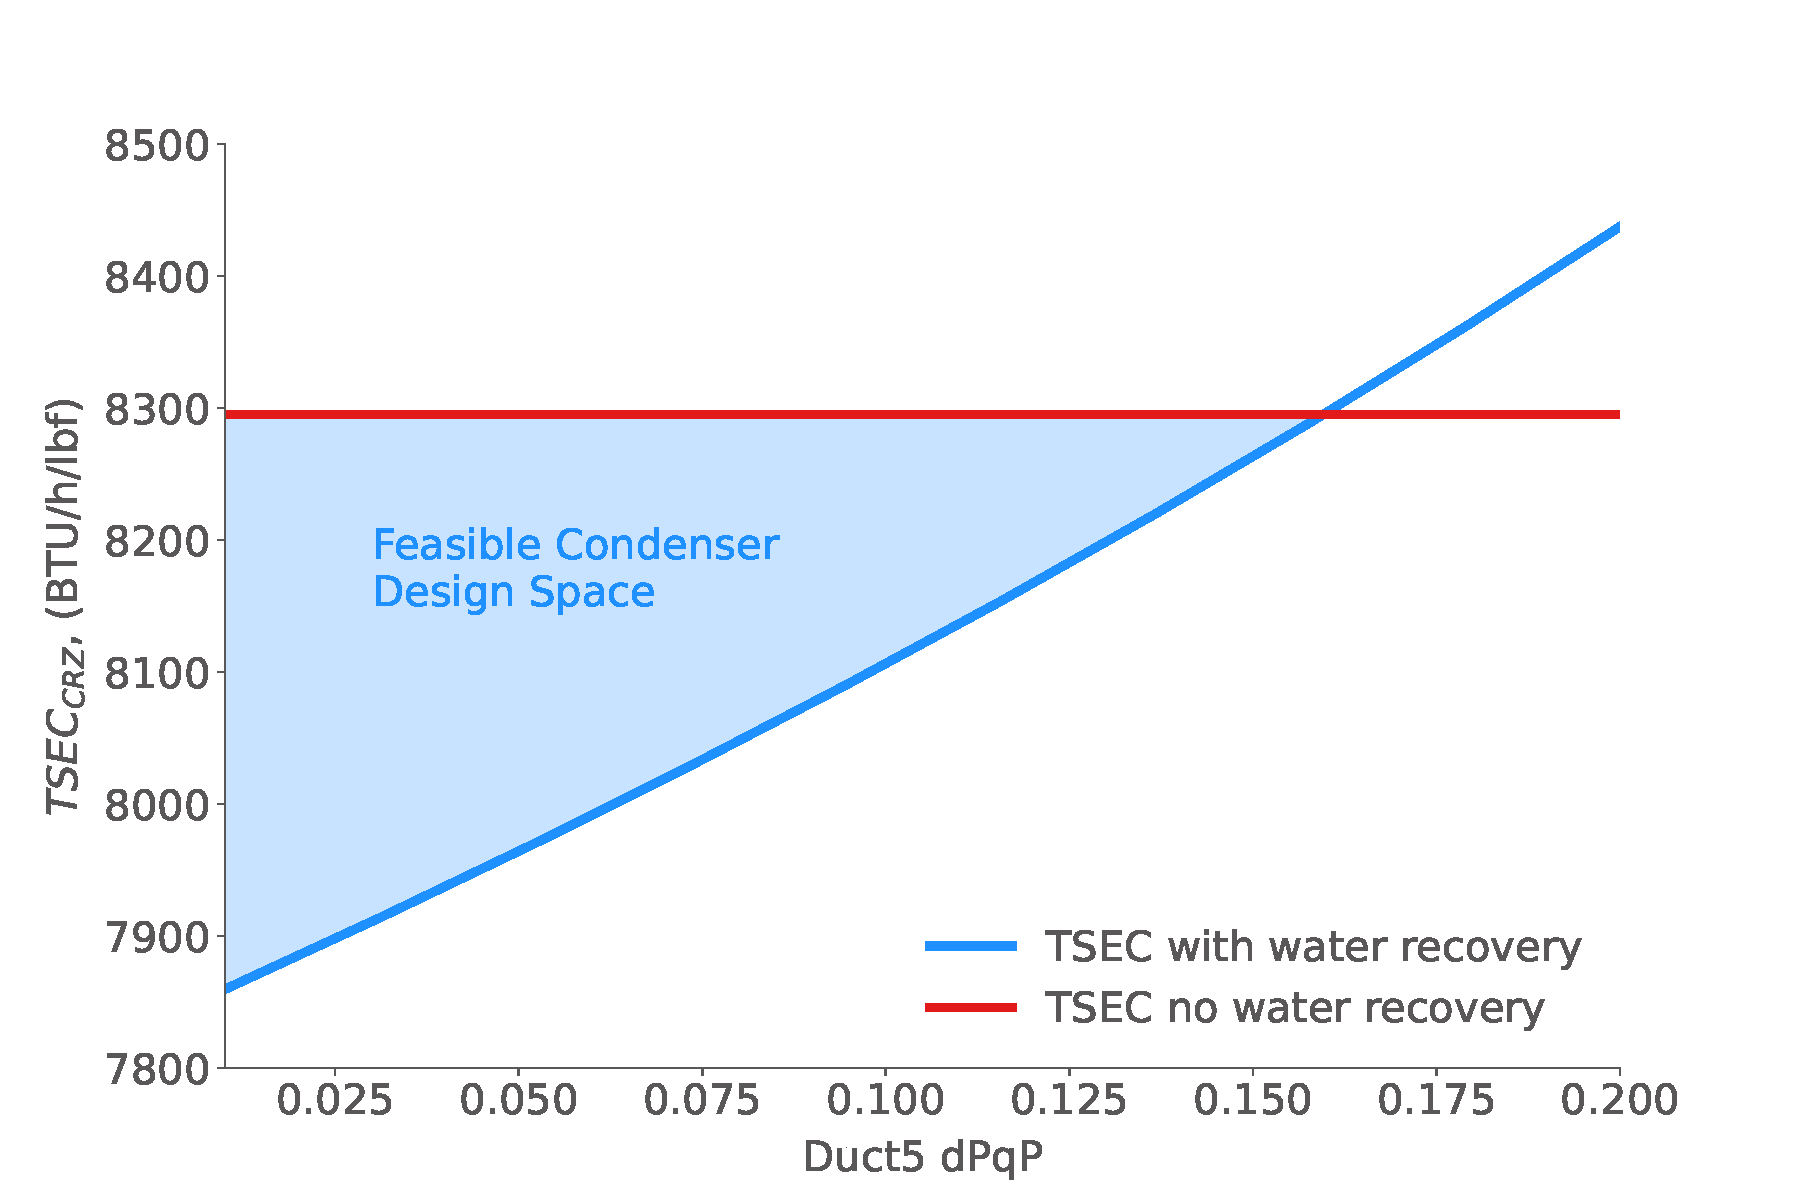
\includegraphics[width=\textwidth]{N3_dpqp.pdf}
        \caption{Pressure loss sweep of Duct5 which is just upstream of the water vapor extractor component.
            The figure shows the optimized TSEC values for varying levels of pressure loss due to the condensation of water compared to the optimization problem without water recovery.
            This shows the working space available for designing a water condenser while still gaining the benefits of water recovery.}
        \label{fig:dpqp_sweep}
    \end{subfigure}
    \hspace{2pt}
    \begin{subfigure}[t]{0.49\textwidth}
        % [x] TODO: AL-PA, Rotate the y-axis label to go vertically to save space
        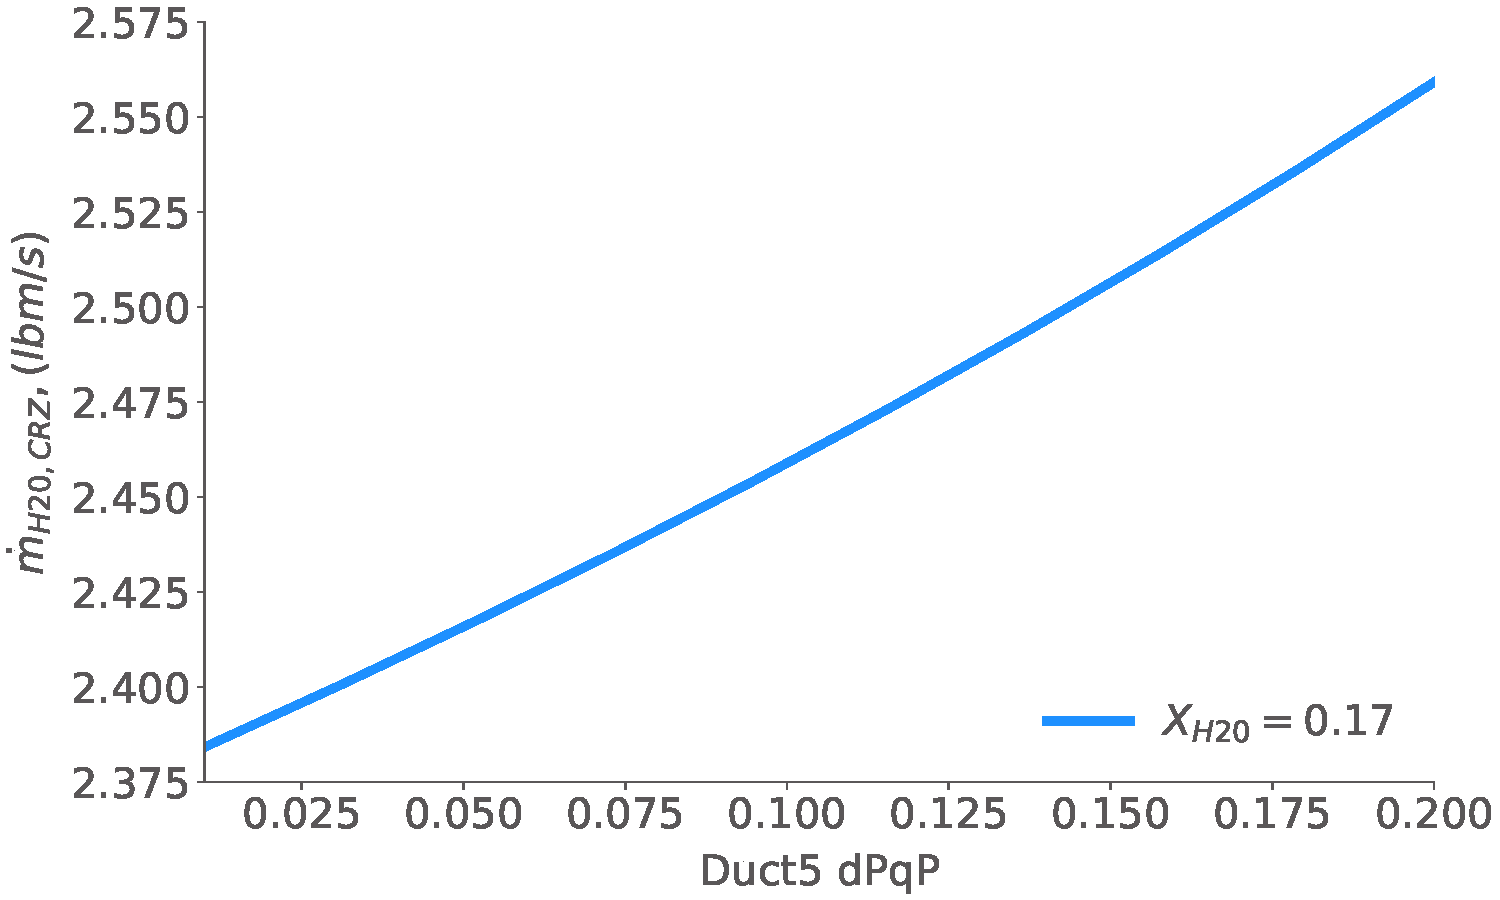
\includegraphics[width=\textwidth]{N3_wdot.pdf}
        \caption{Pressure loss sweep of Duct5 which is just upstream of the water vapor extractor component.
            The figure shows the resulting total available water in the exhaust stream for varying levels of pressure loss in the extractor flow path.
            The engine was optimized with the water recovery upper bound of 17\%.
        }
        \label{fig:dpqp_wdot}
    \end{subfigure}
    \caption{}
    \label{fig:dpqp_study}
\end{figure}
% From Figure~\ref{fig:dpqp_sweep}, we can see the design space in which the closed-loop water recovery model is feasible.
The breakeven point where water recovery is no longer beneficial occurs at a pressure loss of roughly 0.16, or 16\%.
This estimate is based on an ideal condenser that can achieve the optimal water extraction for a given pressure loss.
In reality, losses due to inefficiencies further reduce the size of the feasible space.
% The water recovery model will offer efficiency improvements up until about $\rm{dPqP} = 0.16$.
% A value of $\rm{dPqP} = 0.16$ means that a 16\% loss of pressure from the condenser is allowed assuming the maximum water recovery fraction of 17\% for \ce{H2}.
% This improvement design space would be reduced if only a smaller fraction of water recovered could be obtained.
% [x] TODO: AL-PA, Re-write this part to match the new figure that shows the mass flow of water extracted (per our slack convo)
The water flow rate extracted from the core stream as a function of the same pressure loss is shown in Figure~\ref{fig:dpqp_wdot}.
% Figure~\ref{fig:dpqp_wdot} shows that the optimizer finds designs that increase the available water in the core stream.
Since the water recovery fraction is always pushed to 17\%, the optimizer increases the recovered water mass flow rate to overcome the pressure loss.
This effect helps the engine increase the feasible design space in Figure~\ref{fig:dpqp_sweep}.
The hydrogen fuel would serve a double purpose in this cycle.
The cold hydrogen fuel can be used as a heat sink for the condenser and then injected into the combustor at a higher temperature, further improving efficiency~\cite{Boggia2002}.

% Motivation: space to work with hydrogen, benefits of water injection, benefits of H2 (a lot of water, no tanks, de-mineralized water)
\section{Conclusion}
\label{sec:conc}
In this paper, we describe a novel closed-loop water recirculation system for commercial aviation engines.
The water recirculation system was designed and implemented within the N+3 ultra-high bypass engine model.
We presented the results of four optimization problems demonstrating the use of this technology within pyCycle for Jet-A and hydrogen fuels.

The water recirculation system introduces two pyCycle components, namely the water extractor and injector, that form a continuous closed-loop feedback cycle in the engine.
% We then described the multipoint design problem and how it is used to design an aircraft engine to meet the operating requirements at different flight regimes.
% The optimization problem is then introduced with constraints on the thrust and overall engine size at the design point.
We optimize the engine cycle considering Jet-A and hydrogen fuels with and without water recovery.
The objective is to minimize fuel mass flow rate subject to net thrust and fan diameter constraints.
% The design variables used are thermodynamic design variables describing the temperatures, pressures, and velocities within the engine.
% An additional design variable controlling how much water is recirculated is added at the cruise point to improve the fuel burn.
% The optimization problem was solved for four cases: with Jet-A or hydrogen fuel, and with or without water recirculation.
% The results from the optimization problems show temperature, thrust, and efficiency improvements for hydrogen as a fuel and even further improvements with water circulation.
The results show that optimal hydrogen-fueled engines with water recirculation are more efficient than standard Jet-A with no water recovery.
We demonstrate that the increased availability of water from hydrogen combustion proves the viability of this concept.
Additionally, hydrogen combustion eliminates carbon emissions and the lean fuel-to-air ratios result in cooler turbine inlet temperatures compared to Jet-A.
% Thermal reductions with hydrogen and water recirculation will improve the lifetime of the engine which would reduce maintenance and overall costs.
% Between the two fuels, we see similar values of the engine performance metric, TSEC.
% Significant energy efficiency gains are seen with water recirculation which would improve the overall costs of the engine during its operational lifecycle.
% At the same water recovery fraction, hydrogen with water recirculation could achieve a lower TSEC value.

We performed a design space study to understand the technology requirements for a condenser that might operate in the proposed water recovery system.
% There are technological obstacles to overcome in order to implement this water recirculation system in a modern turbofan engine.
% The main obstacle would be how to design a condenser that can recover a portion of the exhaust water without a excessive drag pressure losses.
% Therefore, a condenser design space study was completed to show the feasible design space for such a condenser.
The results showed that a hydrogen-fueled cycle with water recovery can sustain a pressure loss of 16\% across a condenser before the efficiency benefits diminish.
% The results of the study showed that at the maximum possible water recovery fraction for hydrogen quite a large pressure loss can be imposed before the improvements are canceled out.
% Furthermore, using hydrogen as the fuel allows for designs that are not available for an engine using Jet-A.
% [x] TODO: AL-PA, I suggest you bolster the discussion of these two sentences in the results section and maybe add a citation?
The thermal properties of hydrogen provide a heat sink and thus a readily available resource for water condensation within the condenser.
The hydrogen fuel absorbs heat and is then used in the combustion process, further improving engine efficiency.
% The novel water recovery system shows promising efficiency results when used with hydrogen fuel.
Hydrogen-fueled UHBR turbofan engines can be more efficient than Jet-A counterparts when optimized considering water recovery.
Taking advantage of the beneficial properties of hydrogen is paramount for new engine technologies that can reduce emissions while improving performance.
% This water recovery system provides a potential avenue for hydrogen engine design that could help overcome the technological issues associated with hydrogen as a fuel.

\section{Acknowledgements}
\noindent
We would like to thank Justin Gray for his support in the development of the water recovery pyCycle models.

\bibliography{mdolab,references}

\end{document}